\documentclass[11pt,a4paper]{report}
% ============================================================
%  Shared preamble: colours, typography, boxes, tables, UML/TikZ styles
% ============================================================
\usepackage[T1]{fontenc}
\usepackage[utf8]{inputenc}
\usepackage{mathpazo}
\usepackage[scaled=0.92]{helvet}
\usepackage[a4paper,margin=2.4cm,headheight=15pt]{geometry}
\usepackage[table,dvipsnames]{xcolor}
\usepackage{microtype}
\usepackage{amsmath}
\usepackage{graphicx}
\usepackage{array,booktabs,longtable,tabularx,multirow}
\usepackage{enumitem}
\usepackage{float}
\usepackage[font=small,labelfont={bf,color=navy},textfont=it,skip=6pt]{caption}
\usepackage{fancyhdr}
\usepackage{titlesec}
\usepackage{listings}
\usepackage{tikz}
\usetikzlibrary{arrows.meta,positioning,shapes.geometric,shapes.multipart,shapes.misc,fit,backgrounds,calc,decorations.pathreplacing,patterns}
\usepackage{pgfgantt}
\usepackage[most]{tcolorbox}
\usepackage[colorlinks=true,linkcolor=teal,urlcolor=teal,citecolor=teal]{hyperref}

% ---------- Colour palette ----------
\definecolor{navy}{HTML}{0B2545}
\definecolor{teal}{HTML}{0E8F9C}
\definecolor{tealdark}{HTML}{0A6B75}
\definecolor{amber}{HTML}{F2A33A}
\definecolor{coral}{HTML}{D9534F}
\definecolor{violet}{HTML}{6C4FA1}
\definecolor{leaf}{HTML}{3E9B5F}
\definecolor{mist}{HTML}{EEF3F8}
\definecolor{mint}{HTML}{DDF3F1}
\definecolor{sand}{HTML}{FDF1DC}
\definecolor{blush}{HTML}{FBE3E1}
\definecolor{lilac}{HTML}{E9E3F5}
\definecolor{slate}{HTML}{4A5568}
\definecolor{rowgray}{HTML}{F3F6FA}

% ---------- Project macros (change here only) ----------
\newcommand{\projname}{DocuMind AI}
\newcommand{\projfull}{Intelligent Document Processing and Automated ERP Ingestion System}
\newcommand{\studentname}{Tuheu Tchoubi Pempeme Moussa Fahdil}
\newcommand{\supervisorname}{[Supervisor name -- to be completed]}
\newcommand{\docversion}{2.0}
\newcommand{\docdate}{October 2026}

% ---------- Headings ----------
\titleformat{\chapter}[display]
  {\sffamily\bfseries\color{navy}}
  {\vspace*{-0.5cm}\color{teal}\fontsize{54}{54}\selectfont\thechapter}
  {0.2cm}
  {\Huge}
  [\vspace{2pt}{\color{teal}\titlerule[2.2pt]}]
\titlespacing*{\chapter}{0pt}{0pt}{26pt}
\titleformat{\section}{\sffamily\Large\bfseries\color{navy}}{\color{teal}\thesection}{0.6em}{}
\titleformat{\subsection}{\sffamily\large\bfseries\color{tealdark}}{\thesubsection}{0.6em}{}
\titleformat{\subsubsection}{\sffamily\normalsize\bfseries\color{slate}}{\thesubsubsection}{0.6em}{}
\titlespacing*{\section}{0pt}{16pt}{6pt}
\titlespacing*{\subsection}{0pt}{12pt}{4pt}

% ---------- Header / footer ----------
\pagestyle{fancy}
\fancyhf{}
\renewcommand{\headrulewidth}{0.6pt}
\renewcommand{\headrule}{\hbox to\headwidth{\color{teal}\leaders\hrule height \headrulewidth\hfill}}
\renewcommand{\footrulewidth}{0pt}
\fancyhead[L]{\small\sffamily\color{navy}\projname}
\fancyhead[R]{\small\sffamily\color{slate}\nouppercase{\leftmark}}
\fancyfoot[C]{\small\sffamily\color{slate}\thepage}
\fancypagestyle{plain}{\fancyhf{}\fancyfoot[C]{\small\sffamily\color{slate}\thepage}\renewcommand{\headrulewidth}{0pt}}

% ---------- Lists, spacing ----------
\setlist{itemsep=2pt,topsep=4pt,parsep=0pt}
\setlist[itemize]{label=\textcolor{teal}{\textbullet}}
\setlist[enumerate]{label=\textcolor{teal}{\bfseries\arabic*.}}
\setlength{\parindent}{0pt}
\setlength{\parskip}{6pt}
\renewcommand{\arraystretch}{1.25}
\setcounter{tocdepth}{2}

% ---------- Call-out boxes ----------
\tcbset{calloutbase/.style={enhanced,breakable,sharp corners,boxrule=0pt,leftrule=3.5pt,
  left=8pt,right=8pt,top=6pt,bottom=6pt,fonttitle=\sffamily\bfseries,coltitle=navy,
  attach boxed title to top left={yshift=-2mm},
  boxed title style={colback=white,boxrule=0pt,top=0pt,bottom=0pt,left=0pt}}}
\newtcolorbox{infobox}[1][Note]{calloutbase,colback=mint,colframe=teal,title={#1}}
\newtcolorbox{warnbox}[1][Important]{calloutbase,colback=sand,colframe=amber,title={#1}}
\newtcolorbox{statusbox}[1][Status]{calloutbase,colback=lilac,colframe=violet,title={#1}}
\newtcolorbox{goalbox}[1][Goal]{calloutbase,colback=mist,colframe=navy,title={#1}}

% ---------- Tables ----------
\newcolumntype{L}[1]{>{\raggedright\arraybackslash}p{#1}}
\newcolumntype{C}[1]{>{\centering\arraybackslash}p{#1}}
\newcommand{\hdr}[1]{\textcolor{white}{\sffamily\bfseries #1}}
\newcommand{\tblstart}{\rowcolors{2}{white}{rowgray}\arrayrulecolor{teal!60}}
\newcommand{\hdrrow}{\rowcolor{navy}}
\newcommand{\must}{\textcolor{coral}{\sffamily\bfseries Must}}
\newcommand{\should}{\textcolor{amber!85!black}{\sffamily\bfseries Should}}
\newcommand{\could}{\textcolor{tealdark}{\sffamily\bfseries Could}}
\newcommand{\wont}{\textcolor{slate}{\sffamily\bfseries Won't (now)}}
\newcommand{\done}{\textcolor{leaf}{\sffamily\bfseries Done}}
\newcommand{\inprog}{\textcolor{amber!85!black}{\sffamily\bfseries Partial}}
\newcommand{\todo}{\textcolor{slate}{\sffamily\bfseries Planned}}
\newcommand{\code}[1]{\texttt{\small #1}}

% ---------- Code listings ----------
\lstdefinestyle{docu}{basicstyle=\ttfamily\footnotesize,backgroundcolor=\color{mist},
  frame=l,rulecolor=\color{teal},framerule=3pt,xleftmargin=10pt,framexleftmargin=6pt,
  keywordstyle=\color{tealdark}\bfseries,commentstyle=\color{slate}\itshape,
  stringstyle=\color{violet},showstringspaces=false,breaklines=true,columns=fullflexible,
  aboveskip=8pt,belowskip=8pt}
\lstset{style=docu}

% ---------- TikZ / UML styles ----------
\tikzset{
  every picture/.append style={font=\sffamily\small},
  box/.style={rectangle,rounded corners=3pt,draw=navy,line width=0.7pt,fill=mist,align=center,
              minimum height=0.8cm,inner sep=4pt},
  boxT/.style={box,fill=mint,draw=tealdark},
  boxA/.style={box,fill=sand,draw=amber!80!black},
  boxV/.style={box,fill=lilac,draw=violet},
  boxC/.style={box,fill=blush,draw=coral},
  boxN/.style={box,fill=navy,draw=navy,text=white},
  arr/.style={-{Stealth[length=2.6mm,width=1.9mm]},line width=0.7pt,color=navy},
  arrd/.style={-{Stealth[length=2.6mm,width=1.9mm]},line width=0.7pt,color=slate,dashed},
  lbl/.style={font=\sffamily\scriptsize,color=slate,fill=white,inner sep=1.2pt},
  state/.style={rectangle,rounded corners=8pt,draw=tealdark,fill=mint,line width=0.8pt,
                minimum width=2.5cm,minimum height=0.9cm,align=center,font=\sffamily\footnotesize\bfseries},
  stateA/.style={state,fill=sand,draw=amber!80!black},
  stateC/.style={state,fill=blush,draw=coral},
  stateV/.style={state,fill=lilac,draw=violet},
  initial/.style={circle,fill=navy,minimum size=0.35cm,inner sep=0pt},
  final/.style={circle,draw=navy,line width=0.9pt,minimum size=0.5cm,inner sep=0pt,
                path picture={\fill[navy] (path picture bounding box.center) circle (0.17cm);}},
  uclass/.style={rectangle split,rectangle split parts=3,draw=navy,line width=0.8pt,fill=white,
                 font=\sffamily\scriptsize,text width=3.55cm,inner sep=3pt,align=left,
                 rectangle split part fill={mint,white,white}},
  uclass2/.style={rectangle split,rectangle split parts=2,draw=navy,line width=0.8pt,fill=white,
                 font=\sffamily\scriptsize,text width=3.55cm,inner sep=3pt,align=left,
                 rectangle split part fill={mint,white}},
  uiface/.style={uclass2,rectangle split part fill={sand,white}},
  uenum/.style={uclass2,rectangle split part fill={lilac,white}},
  ucase/.style={ellipse,draw=tealdark,fill=mint,line width=0.7pt,align=center,
                font=\sffamily\scriptsize,minimum height=0.8cm,inner xsep=3pt},
  lifeline/.style={dashed,color=slate,line width=0.6pt},
  msg/.style={-{Stealth[length=2.4mm,width=1.7mm]},line width=0.65pt,color=navy},
  ret/.style={-{Stealth[length=2.4mm,width=1.7mm]},line width=0.65pt,color=slate,dashed},
}
% stick-figure actor: \actor{name}{x}{y}{label}
\newcommand{\actor}[4]{%
  \begin{scope}[shift={(#2,#3)},color=navy,line width=0.9pt]
    \draw[fill=sand] (0,0.95) circle (0.2);
    \draw (0,0.75)--(0,0.1) (-0.35,0.55)--(0.35,0.55) (0,0.1)--(-0.28,-0.4) (0,0.1)--(0.28,-0.4);
    \node[font=\sffamily\scriptsize\bfseries,text=navy,align=center,below] (#1) at (0,-0.38) {#4};
  \end{scope}}
% class-name helper (centred bold)
\newcommand{\cname}[1]{\centerline{\bfseries #1}}
\newcommand{\stereo}[1]{\guillemotleft\,#1\,\guillemotright}

\hypersetup{pdftitle={DocuMind AI - Phase 2 System Design Specification},pdfauthor={Tuheu Tchoubi Pempeme Moussa Fahdil}}
\begin{document}
\begin{titlepage}
\newgeometry{margin=0cm}
\thispagestyle{empty}
\begin{tikzpicture}[remember picture,overlay]
  \fill[navy] (current page.north west) rectangle ([yshift=-17.5cm]current page.north east);
  \fill[teal] ([yshift=-17.5cm]current page.north west) rectangle ([yshift=-17.9cm]current page.north east);
  \fill[amber] ([yshift=-17.9cm]current page.north west) rectangle ([yshift=-18.1cm]current page.north east);
  % decorative document / network motif
  \begin{scope}[shift={([xshift=-8.2cm,yshift=-4.6cm]current page.north east)},opacity=0.9]
    \draw[teal!70,line width=1pt,fill=white!8!navy] (0,0) rectangle (2.6,3.4);
    \foreach \y in {0.5,0.9,1.3,1.7,2.1} {\draw[teal!70,line width=0.8pt] (0.3,\y) -- (2.3,\y);}
    \draw[amber,line width=1.4pt,fill=amber!25!navy] (0.3,2.5) rectangle (1.5,2.9);
    \draw[-{Stealth},amber,line width=1.2pt] (2.8,1.7) -- (4.0,1.7);
    \draw[teal!70,line width=1pt,fill=white!8!navy] (4.2,0.9) rectangle (5.3,2.5);
    \foreach \y in {1.2,1.6,2.0} {\draw[teal!70,line width=0.8pt] (4.4,\y) -- (5.1,\y);}
  \end{scope}
  \node[anchor=west,text=white,font=\sffamily\bfseries\fontsize{40}{44}\selectfont] at ([xshift=2.4cm,yshift=-9.3cm]current page.north west) {\projname};
  \node[anchor=west,text=teal!30,font=\sffamily\fontsize{15}{19}\selectfont,text width=15cm] at ([xshift=2.4cm,yshift=-11.5cm]current page.north west) {Intelligent Document Processing and\\ Automated ERP Ingestion System};
  \node[anchor=west,text=white,font=\sffamily\small,text width=15cm] at ([xshift=2.4cm,yshift=-13.7cm]current page.north west) {Phase 2 -- System Design and Architecture};
  \node[anchor=west,text=amber,font=\sffamily\bfseries\footnotesize] at ([xshift=2.4cm,yshift=-15.3cm]current page.north west) {ARCHITECTURE \ $\cdot$ \ DATABASE \ $\cdot$ \ WORKFLOW \ $\cdot$ \ API \ $\cdot$ \ INTERFACE \ $\cdot$ \ SECURITY};
  \node[anchor=west,text=white!70,font=\sffamily\scriptsize] at ([xshift=2.4cm,yshift=-3.0cm]current page.north west) {ICT UNIVERSITY \ $\cdot$ \ FACULTY OF ICT \ $\cdot$ \ DEPARTMENT OF COMPUTER SCIENCE};
\end{tikzpicture}
\begin{tikzpicture}[remember picture,overlay]
\node[anchor=north west,text width=15.5cm,font=\sffamily\small] at ([xshift=2.4cm,yshift=-19.3cm]current page.north west) {%
\begin{tabular}{@{}L{3.2cm}L{11cm}@{}}
\textcolor{teal}{\bfseries Student}   & \studentname\\
\textcolor{teal}{\bfseries Programme} & B.Sc. Computer Science, final-year project\\
\textcolor{teal}{\bfseries Supervisor}& \supervisorname\\
\textcolor{teal}{\bfseries Institution}& The ICT University, Cameroon\\
\textcolor{teal}{\bfseries Version}    & 1.0 \ -- \docdate\\
\end{tabular}};
\end{tikzpicture}
\restoregeometry
\end{titlepage}

\pagenumbering{roman}
\chapter*{Document Control}
\addcontentsline{toc}{chapter}{Document Control}
\tblstart\small
\begin{longtable}{L{3.4cm}L{11.0cm}}
\hdrrow \hdr{Item} & \hdr{Description}\\ \endhead
Document & \projname{} -- Phase 2: System Design and Architecture.\\
Version & 1.0 (October 2026).\\
Deliverable & Design specification covering user stories US-06 to US-11: system architecture, database design, document-processing workflow, REST API, user interface, security and ERP integration.\\
Companion files & \texttt{schema.sql} (MySQL schema), \texttt{openapi.yaml} (API contract) and \texttt{gen\_tables.py} (generates the tables of this document from those two files).\\
Builds on & \emph{Phase 1 Requirements Specification} (requirements FR-01 to FR-22, NFR-01 to NFR-10, business rules BR-1 to BR-6).\\
Status & \textbf{Draft for supervisor review.} Decisions that remain open are listed in Section~\ref{sec:p2open}.\\
Honesty note & This is a design. The two health endpoints are the only API code that exists. Section~\ref{sec:p2verified} states exactly what was verified and what was not.\\
\hline
\end{longtable}
\clearpage
\tableofcontents
\clearpage
\listoffigures
\clearpage
\pagenumbering{arabic}
\setcounter{page}{1}

\newcommand{\nTables}{11}\newcommand{\nColumns}{106}\newcommand{\nOps}{24}\newcommand{\nPaths}{22}\newcommand{\nSchemas}{21}

\chapter{Overview of Phase 2}\label{ch:p2overview}
\section{Goal}
Phase 2 answers one question: \emph{how will the frontend, backend, database, OCR engine and ERP integration work together?} The Phase 1 requirements said what the system must do. This phase decides how it is built, in enough detail that Phase 3 onward can implement it without guessing.

\section{User stories covered}
The six stories below come from the project Kanban board. Each one is closed by a chapter of this document and, where useful, by a file that a program can check.

{\tblstart\small
\begin{longtable}{L{1.4cm}L{5.2cm}L{1.6cm}L{5.6cm}}
\hdrrow \hdr{Story} & \hdr{Title} & \hdr{Chapter} & \hdr{Main deliverable}\\ \endhead
US-06 & Design the system architecture & \ref{ch:p2arch} & Layered architecture, technology decisions, module rules, deployment views.\\
US-07 & Design the database & \ref{ch:p2db} & \texttt{schema.sql}: \nTables{} tables, \nColumns{} columns, keys, checks, indexes, audit trigger.\\
US-08 & Design the document-processing workflow & \ref{ch:p2flow} & Stage table, state machine, validation and retry rules.\\
US-09 & Design the REST API & \ref{ch:p2api} & \texttt{openapi.yaml}: \nOps{} operations, \nSchemas{} schemas, error model.\\
US-10 & Design the user interface & \ref{ch:p2ui} & Screen map, wireframes, state table.\\
US-11 & Define security and ERP integration & \ref{ch:p2sec} & Threat and control table, ERP adapter design, mapping and retry policy.\\
\hline
\end{longtable}}

\section{Main design decisions at a glance}
{\tblstart\small
\begin{longtable}{L{3.6cm}L{4.6cm}L{5.6cm}}
\hdrrow \hdr{Topic} & \hdr{Decision} & \hdr{Reason}\\ \endhead
Backend shape & One FastAPI application with separated modules. & Fewer moving parts for a single developer; services can be extracted later.\\
Database & MySQL 8 with SQLAlchemy 2 and Alembic migrations. & Project requirement; migrations make schema changes repeatable.\\
Processing & Asynchronous: the upload returns \texttt{202} at once. & OCR is slow; the user must not wait on a request.\\
OCR & Behind an \texttt{OcrEngine} interface with two implementations: Tesseract and the custom CRNN model. & Fair comparison and a working fallback.\\
ERP & Behind an \texttt{ErpAdapter} interface with a mock and an Odoo implementation. & The mock lets the project run without Odoo access.\\
Review & Mandatory before any ERP submission. & Business rule BR-1.\\
Identity & Short-lived bearer token; role checked in the backend on every request. & The browser is never trusted to enforce permissions.\\
History & Every run, correction and ERP attempt is kept. & Business rules BR-5 and BR-6; auditing.\\
\hline
\end{longtable}}

\section{What was checked}\label{sec:p2verified}
\begin{statusbox}[Verification status]
\textbf{Checked.} \texttt{schema.sql} was loaded into a real database engine (MariaDB 10.11, which is MySQL-compatible) and nine invalid inserts were rejected as designed (Section~\ref{sec:p2dbtests}). \texttt{openapi.yaml} passes an OpenAPI 3.0 validator. The document statuses in the API and in the database are identical. The column dictionary and endpoint catalogue in this document are \emph{generated} from those two files.\\[3pt]
\textbf{Not checked.} The schema has not been run on MySQL 8.0 itself. No endpoint other than \texttt{/health} and \texttt{/health/db} exists in code. The screens are wireframes, not a running interface. Nothing has been tried against Odoo. Timing, confidence thresholds and retry values are planning values, not measurements.
\end{statusbox}

% =====================================================================
\chapter{System Architecture}\label{ch:p2arch}
\emph{Story US-06.} The chapter fixes the frontend, backend and database technologies, shows the OCR pipeline and the ERP integration in one diagram, and states the rules that keep the modules separate.

\section{Scope and context}
\projname{} sits between people who hold invoices and the ERP that must record them. Three kinds of people use it (operator, reviewer, administrator). One external system receives data from it (the ERP). Everything else, including OCR, runs inside the system boundary.

\section{Layered architecture}
\begin{figure}[H]\centering
\resizebox{\textwidth}{!}{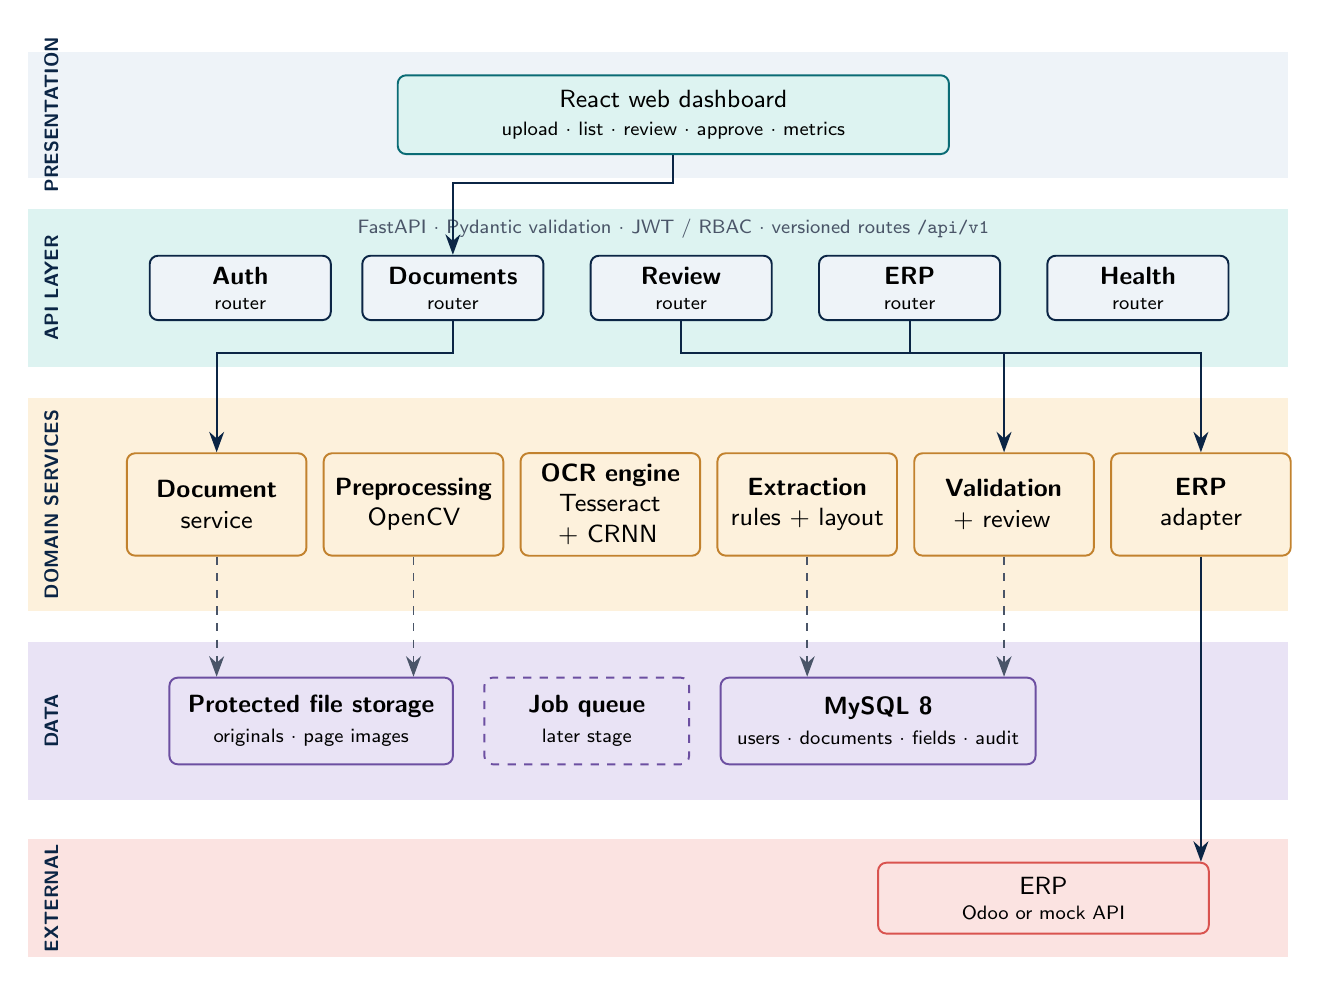
\begin{tikzpicture}[x=1cm,y=1cm]
% layer bands
\fill[mist]  (0,8.5) rectangle (16,10.1);
\fill[mint]  (0,6.1) rectangle (16,8.1);
\fill[sand]  (0,3.0) rectangle (16,5.7);
\fill[lilac] (0,0.6) rectangle (16,2.6);
\fill[blush] (0,-1.4) rectangle (16,0.1);
\node[rotate=90,font=\sffamily\scriptsize\bfseries,text=navy] at (0.3,9.3) {PRESENTATION};
\node[rotate=90,font=\sffamily\scriptsize\bfseries,text=navy] at (0.3,7.1) {API LAYER};
\node[rotate=90,font=\sffamily\scriptsize\bfseries,text=navy] at (0.3,4.35) {DOMAIN SERVICES};
\node[rotate=90,font=\sffamily\scriptsize\bfseries,text=navy] at (0.3,1.6) {DATA};
\node[rotate=90,font=\sffamily\scriptsize\bfseries,text=navy] at (0.3,-0.65) {EXTERNAL};
% presentation
\node[boxT,minimum width=7cm,minimum height=1cm] (ui) at (8.2,9.3) {React web dashboard\\[-1pt]\scriptsize upload $\cdot$ list $\cdot$ review $\cdot$ approve $\cdot$ metrics};
% api
\foreach \x/\t in {2.3/Auth,5.0/Documents,7.9/Review,10.8/ERP,13.7/Health}{
  \node[box,minimum width=2.3cm] (r\t) at (\x+0.4,7.1) {\textbf{\t}\\[-2pt]\scriptsize router};}
\node[font=\sffamily\scriptsize,text=slate] at (8.2,7.85) {FastAPI $\cdot$ Pydantic validation $\cdot$ JWT / RBAC $\cdot$ versioned routes \texttt{/api/v1}};
% domain
\foreach \x/\t/\s in {2.3/Document/service,4.95/Pre-/processing,7.6/OCR/engine,10.25/Extraction/rules,12.9/Validation/+ review,15.0/ERP/adapter}{}
\node[boxA,text width=2.0cm,minimum height=1.3cm] (sdoc) at (2.4,4.35)  {\textbf{Document}\\service};
\node[boxA,text width=2.0cm,minimum height=1.3cm] (spre) at (4.9,4.35)  {\textbf{Preprocessing}\\OpenCV};
\node[boxA,text width=2.0cm,minimum height=1.3cm] (socr) at (7.4,4.35)  {\textbf{OCR engine}\\Tesseract\\+ CRNN};
\node[boxA,text width=2.0cm,minimum height=1.3cm] (sext) at (9.9,4.35)  {\textbf{Extraction}\\rules + layout};
\node[boxA,text width=2.0cm,minimum height=1.3cm] (sval) at (12.4,4.35) {\textbf{Validation}\\+ review};
\node[boxA,text width=2.0cm,minimum height=1.3cm] (serp) at (14.9,4.35) {\textbf{ERP}\\adapter};
% data
\node[boxV,minimum width=3.6cm,minimum height=1.1cm] (fs) at (3.6,1.6) {\textbf{Protected file storage}\\\scriptsize originals $\cdot$ page images};
\node[boxV,minimum width=2.6cm,minimum height=1.1cm,dashed] (q) at (7.1,1.6) {\textbf{Job queue}\\\scriptsize later stage};
\node[boxV,minimum width=4.0cm,minimum height=1.1cm] (db) at (10.8,1.6) {\textbf{MySQL 8}\\\scriptsize users $\cdot$ documents $\cdot$ fields $\cdot$ audit};
% external
\node[boxC,minimum width=4.2cm,minimum height=0.9cm] (erp) at (12.9,-0.65) {ERP\\[-2pt]\scriptsize Odoo or mock API};
% arrows
\draw[arr] (ui.south) -- ++(0,-0.35) -| (rDocuments.north);
\draw[arr] (rDocuments.south) -- ++(0,-0.4) -| (sdoc.north);
\draw[arr] (rReview.south) -- ++(0,-0.4) -| (sval.north);
\draw[arr] (rERP.south) -- ++(0,-0.4) -| (serp.north);
\draw[arrd] (sdoc.south) -- (sdoc.south |- fs.north);
\draw[arrd] (spre.south) -- (spre.south |- fs.north);
\draw[arrd] (sext.south) -- (sext.south |- db.north);
\draw[arrd] (sval.south) -- (sval.south |- db.north);
\draw[arr]  (serp.south) -- (serp.south |- erp.north);
\end{tikzpicture}
}
\caption{Layered architecture. The React interface calls versioned routers; routers call domain services; services use protected storage, MySQL and, at the bottom, the ERP. The job queue is introduced after the synchronous version works.}\label{fig:p2arch}
\end{figure}

\subsection{Technology decisions (acceptance criteria of US-06)}
{\tblstart\small
\begin{longtable}{L{3.0cm}L{4.1cm}L{6.7cm}}
\hdrrow \hdr{Layer} & \hdr{Choice} & \hdr{Role in the system}\\ \endhead
Web frontend & React with Vite (Node.js toolchain) & Single-page application: sign-in, upload, lists, review workspace, administration.\\
Backend API & FastAPI on Uvicorn & Routing, validation (Pydantic), authentication, orchestration of services.\\
Database & MySQL 8 (InnoDB, utf8mb4) & All structured data: users, documents, runs, fields, reviews, ERP attempts, audit.\\
Data access & SQLAlchemy 2 with PyMySQL; Alembic for migrations & Mapped models and versioned schema changes.\\
Image and PDF handling & OpenCV; PyMuPDF & Render PDF pages, deskew, denoise, binarise.\\
OCR & Tesseract (baseline) and a PyTorch CRNN with CTC (custom) & Text recognition behind one interface.\\
Storage & A private directory first; private object storage later & Original files and page images, never served directly.\\
ERP & Mock service first; Odoo through its external API & Receives approved records.\\
Packaging & Docker and Docker Compose; Kubernetes later & Reproducible setup; local run without Docker stays supported.\\
\hline
\end{longtable}}

\section{Module rules}
The backend is one deployable application. To keep it maintainable the following rules apply.
\begin{enumerate}
\item \textbf{Direction of calls.} Router $\rightarrow$ service $\rightarrow$ repository or adapter. A router never touches the database or the file system directly, and a repository never calls a service.
\item \textbf{Interfaces at the edges.} OCR and ERP are used through interfaces (\texttt{OcrEngine}, \texttt{ErpAdapter}). A new engine or ERP is a new class, not a change to the callers.
\item \textbf{Schemas are not models.} Pydantic schemas describe the API; SQLAlchemy models describe tables. They are kept separate so a table change does not silently change the API.
\item \textbf{One place for state changes.} Document status changes happen in one service function that checks the allowed transitions (Chapter~\ref{ch:p2flow}) and writes the audit event in the same transaction.
\end{enumerate}

\subsection{Planned backend layout}
The folders \texttt{api}, \texttt{core} and \texttt{database} already exist. The others are added as their features are built.
\begin{lstlisting}
backend/app/
  main.py            # application and middleware (exists)
  api/               # routers: health (exists), auth, documents, review, erp, admin
  core/              # settings (exists), security, logging
  database/          # engine and session (exists), migrations
  models/            # SQLAlchemy models, one file per table group
  schemas/           # Pydantic request and response schemas
  services/          # document, workflow, validation, review, audit
  ocr/               # OcrEngine interface, tesseract engine, crnn engine, preprocessing
  erp/               # ErpAdapter interface, mock adapter, odoo adapter
  workers/           # background processing of queued documents
\end{lstlisting}

\section{OCR pipeline and ERP integration in one view}
\begin{figure}[H]\centering
\resizebox{\textwidth}{!}{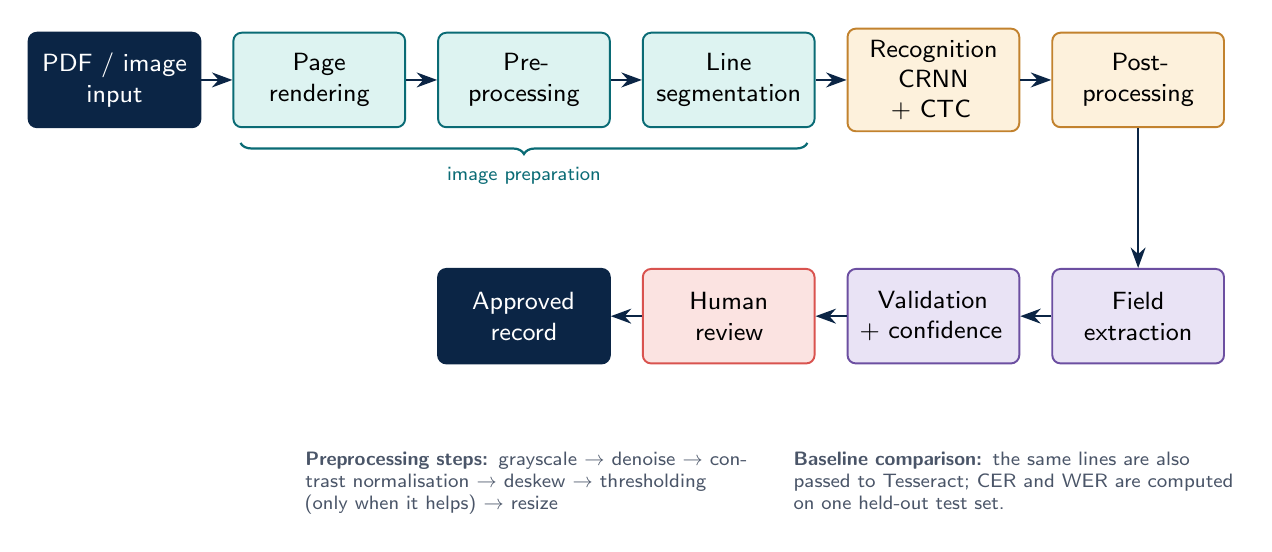
\begin{tikzpicture}[x=1cm,y=1cm,node distance=0.55cm]
\node[boxN,text width=1.9cm,minimum height=1.2cm] (n1) at (1.1,0) {PDF / image\\ input};
\node[boxT,text width=1.9cm,minimum height=1.2cm] (n2) at (3.7,0) {Page\\ rendering};
\node[boxT,text width=1.9cm,minimum height=1.2cm] (n3) at (6.3,0) {Pre-\\processing};
\node[boxT,text width=1.9cm,minimum height=1.2cm] (n4) at (8.9,0) {Line\\ segmentation};
\node[boxA,text width=1.9cm,minimum height=1.2cm] (n5) at (11.5,0) {Recognition\\ CRNN + CTC};
\node[boxA,text width=1.9cm,minimum height=1.2cm] (n6) at (14.1,0) {Post-\\processing};
\node[boxV,text width=1.9cm,minimum height=1.2cm] (n7) at (14.1,-3.0) {Field\\ extraction};
\node[boxV,text width=1.9cm,minimum height=1.2cm] (n8) at (11.5,-3.0) {Validation\\ + confidence};
\node[boxC,text width=1.9cm,minimum height=1.2cm] (n9) at (8.9,-3.0) {Human\\ review};
\node[boxN,text width=1.9cm,minimum height=1.2cm] (n10) at (6.3,-3.0) {Approved\\ record};
\foreach \a/\b in {n1/n2,n2/n3,n3/n4,n4/n5,n5/n6,n6/n7,n7/n8,n8/n9,n9/n10}{\draw[arr] (\a) -- (\b);}
\node[font=\sffamily\scriptsize,text=slate,text width=5.6cm,align=left,anchor=north west] at (3.4,-4.6) {\textbf{Preprocessing steps:} grayscale $\rightarrow$ denoise $\rightarrow$ contrast normalisation $\rightarrow$ deskew $\rightarrow$ thresholding (only when it helps) $\rightarrow$ resize};
\node[font=\sffamily\scriptsize,text=slate,text width=5.6cm,align=left,anchor=north west] at (9.6,-4.6) {\textbf{Baseline comparison:} the same lines are also passed to Tesseract; CER and WER are computed on one held-out test set.};
\draw[decorate,decoration={brace,amplitude=4pt,mirror},color=tealdark,line width=0.8pt] (2.7,-0.8) -- (9.9,-0.8) node[midway,below=5pt,font=\sffamily\scriptsize,text=tealdark] {image preparation};
\end{tikzpicture}
}
\caption{Processing pipeline from upload to ERP submission, with the human review step before the ERP.}\label{fig:p2pipeline}
\end{figure}

\section{Deployment views}
Three ways to run the system are supported, in this order of introduction.
{\tblstart\small
\begin{longtable}{L{3.2cm}L{5.0cm}L{5.6cm}}
\hdrrow \hdr{Mode} & \hdr{What runs where} & \hdr{Used for}\\ \endhead
Local, no Docker & Backend with Uvicorn in a virtual environment; MySQL installed on the PC; React dev server. & Daily development and debugging.\\
Docker Compose & Containers for the backend and MySQL; later a worker and a message broker. & Reproducible demo and clean-machine test (O10).\\
Kubernetes & Deployments for the API and workers; managed or stateful MySQL; secrets and config maps. & Later stage, only if time allows.\\
\hline
\end{longtable}}
\begin{figure}[H]\centering
\resizebox{0.95\textwidth}{!}{\begin{tikzpicture}[x=1cm,y=1cm]
\node[box,fill=mist,minimum width=3.0cm] (br) at (1.6,6.3) {\textbf{Browser}\\\scriptsize React};
\draw[rounded corners=6pt,fill=mint!60,draw=tealdark,line width=0.9pt] (3.7,-0.4) rectangle (14.9,8.1);
\node[font=\sffamily\bfseries\scriptsize,text=tealdark,anchor=north west] at (3.9,8.0) {Docker host (developer PC or VPS) -- network \texttt{idp-net}};
\node[boxT,text width=2.4cm,minimum height=1.5cm] (web) at (5.7,6.0) {\stereo{container}\\\textbf{web}\\\scriptsize nginx + React build};
\node[boxA,text width=2.4cm,minimum height=1.5cm] (api) at (9.2,6.0) {\stereo{container}\\\textbf{backend}\\\scriptsize FastAPI :8000};
\node[boxA,text width=2.4cm,minimum height=1.5cm,dashed] (wrk) at (12.7,6.0) {\stereo{container}\\\textbf{worker}\\\scriptsize OCR jobs (later)};
\node[boxV,text width=2.4cm,minimum height=1.5cm] (db) at (9.2,2.8) {\stereo{container}\\\textbf{mysql}\\\scriptsize MySQL 8 :3306};
\node[boxV,text width=2.4cm,minimum height=1.5cm,dashed] (mq) at (12.7,2.8) {\stereo{container}\\\textbf{rabbitmq}\\\scriptsize broker (later)};
\node[box,fill=white,draw=slate,text width=2.4cm] (v2) at (5.7,2.8) {\stereo{volume}\\ \scriptsize file\_storage};
\node[box,fill=white,draw=slate,text width=2.4cm] (v1) at (9.2,0.4) {\stereo{volume}\\ \scriptsize mysql\_data};
\node[boxC,minimum width=2.4cm] (erp) at (17.3,6.0) {\textbf{ERP}\\\scriptsize Odoo or mock API};
\draw[arr] (br) -- node[lbl,above]{HTTPS} (web);
\draw[arr] (web) -- node[lbl,above]{/api} (api);
\draw[arr] (api) -- node[lbl,right]{SQL} (db);
\draw[arrd] (api.south east) -- (mq.north west);
\draw[arrd] (wrk.south) -- (mq.north);
\draw[arr] (db) -- (v1);
\draw[arr] (api.south west) -- (v2.north east);
\draw[arr] (api.north) -- ++(0,0.5) -| node[lbl,pos=0.25,above]{HTTPS API} (erp.north);
\end{tikzpicture}
}
\caption{Docker Compose deployment (written, not yet run on the developer's machine).}\label{fig:p2compose}
\end{figure}

\section{Architecture decision records}
{\tblstart\small
\begin{longtable}{L{0.9cm}L{3.3cm}L{4.0cm}L{5.6cm}}
\hdrrow \hdr{ID} & \hdr{Decision} & \hdr{Alternative rejected} & \hdr{Consequence}\\ \endhead
A1 & Modular monolith & Microservices from the start & One process to debug; boundaries must be kept by discipline.\\
A2 & Asynchronous processing & Process during the upload request & Needs job state and a worker; the user sees status instead of waiting.\\
A3 & Files outside the database & Store files as BLOBs & Smaller database; storage and database must be backed up together.\\
A4 & UUID identifiers & Auto-increment integers & Identifiers do not reveal volume; slightly larger keys.\\
A5 & Alembic migrations & SQLAlchemy \texttt{create\_all} & Extra setup; every schema change is recorded and reversible.\\
A6 & Mock ERP before Odoo & Wait for Odoo access & Work is not blocked; the adapter must be re-tested against the real ERP.\\
A7 & Roles checked in the backend & Hide buttons in the UI only & Every router needs a role check; UI hiding is only cosmetic.\\
A8 & Keep every processing run & Overwrite results on reprocess & More rows; history satisfies FR-21 and BR-5.\\
\hline
\end{longtable}}

% =====================================================================
\chapter{Database Design}\label{ch:p2db}
\emph{Story US-07.} The chapter identifies the entities, defines tables for documents, extracted fields and review decisions, fixes keys and relationships, and covers processing status and audit history.

\section{Principles}
MySQL stores structured data, not the uploaded files. Each document row holds an opaque storage key, the SHA-256 hash and file metadata. Status values, roles and decisions are restricted by \texttt{CHECK} constraints so that invalid values cannot enter even if the application has a bug. Times are stored in UTC. Nothing that must be remembered for audit is ever updated in place: runs, corrections and ERP attempts are new rows.

\section{Entity-relationship diagram}
\begin{figure}[H]\centering
\resizebox{\textwidth}{!}{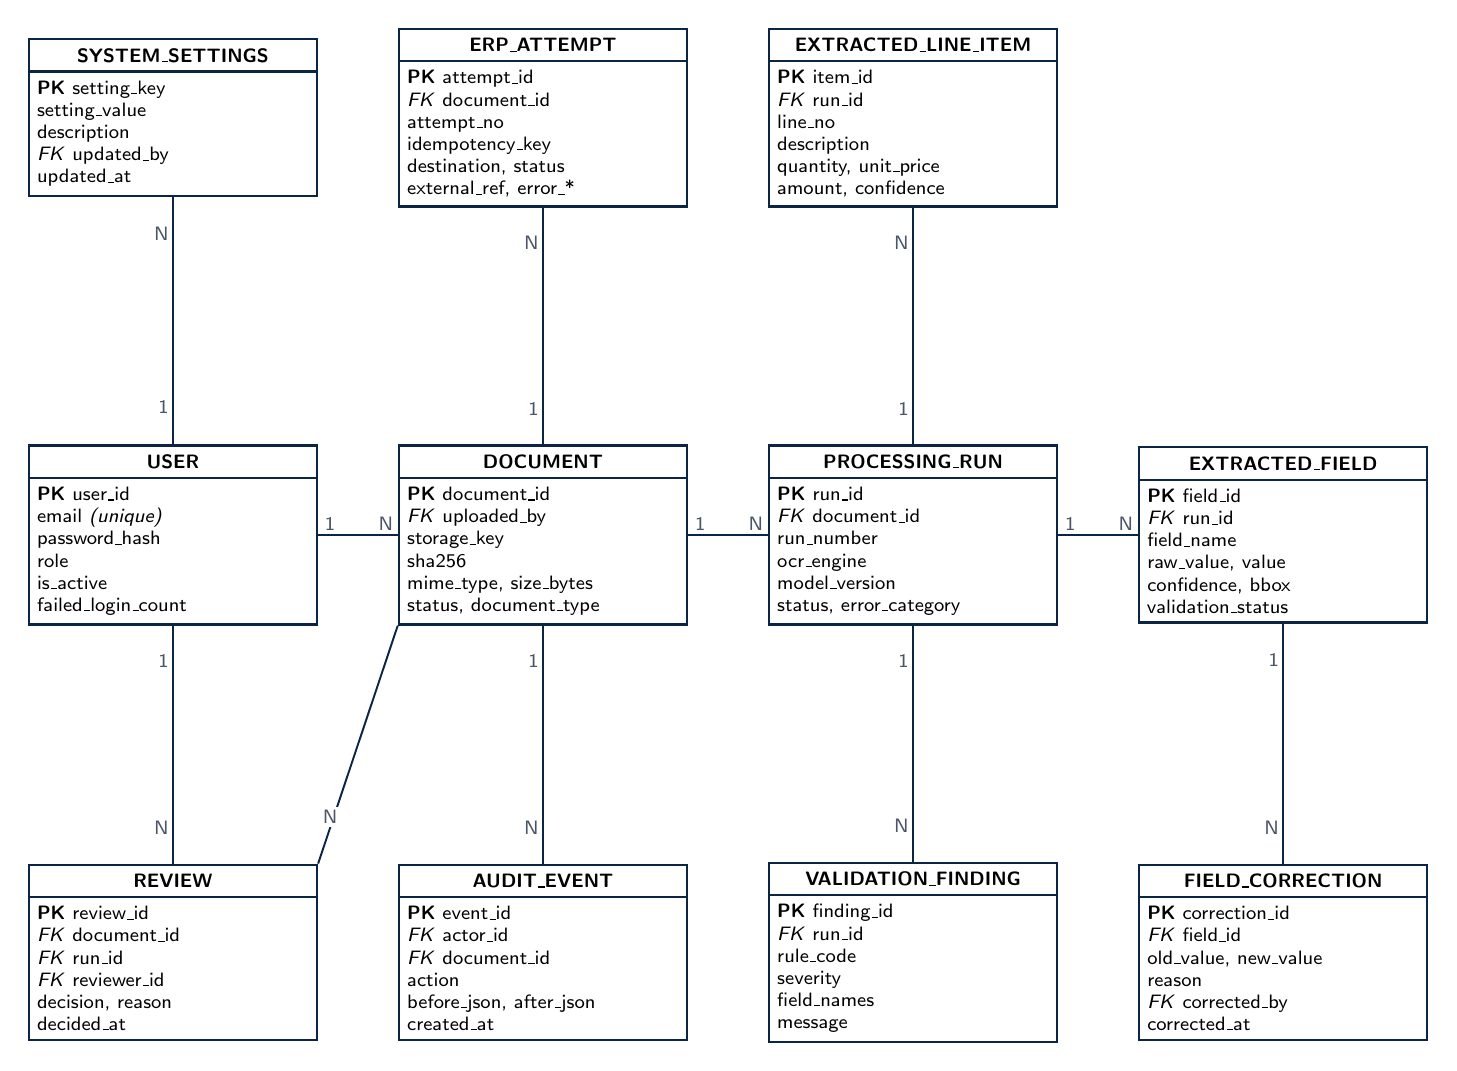
\begin{tikzpicture}[x=1cm,y=1cm,
  ent/.style={uclass2,text width=3.45cm},
  ]
% row 0 (top)
\node[ent] (set) at (0,5.3) {\centerline{{\bfseries SYSTEM\_SETTINGS}}\nodepart{two}
 \textbf{PK} setting\_key\\ setting\_value\\ description\\ \textit{FK} updated\_by\\ updated\_at};
\node[ent] (erp) at (4.7,5.3) {\centerline{{\bfseries ERP\_ATTEMPT}}\nodepart{two}
 \textbf{PK} attempt\_id\\ \textit{FK} document\_id\\ attempt\_no\\ idempotency\_key\\ destination, status\\ external\_ref, error\_*};
\node[ent] (itm) at (9.4,5.3) {\centerline{{\bfseries EXTRACTED\_LINE\_ITEM}}\nodepart{two}
 \textbf{PK} item\_id\\ \textit{FK} run\_id\\ line\_no\\ description\\ quantity, unit\_price\\ amount, confidence};
% row 1
\node[ent] (usr) at (0,0) {\centerline{{\bfseries USER}}\nodepart{two}
 \textbf{PK} user\_id\\ email \textit{(unique)}\\ password\_hash\\ role\\ is\_active\\ failed\_login\_count};
\node[ent] (doc) at (4.7,0) {\centerline{{\bfseries DOCUMENT}}\nodepart{two}
 \textbf{PK} document\_id\\ \textit{FK} uploaded\_by\\ storage\_key\\ sha256\\ mime\_type, size\_bytes\\ status, document\_type};
\node[ent] (run) at (9.4,0) {\centerline{{\bfseries PROCESSING\_RUN}}\nodepart{two}
 \textbf{PK} run\_id\\ \textit{FK} document\_id\\ run\_number\\ ocr\_engine\\ model\_version\\ status, error\_category};
\node[ent] (fld) at (14.1,0) {\centerline{{\bfseries EXTRACTED\_FIELD}}\nodepart{two}
 \textbf{PK} field\_id\\ \textit{FK} run\_id\\ field\_name\\ raw\_value, value\\ confidence, bbox\\ validation\_status};
% row 2
\node[ent] (rev) at (0,-5.3) {\centerline{{\bfseries REVIEW}}\nodepart{two}
 \textbf{PK} review\_id\\ \textit{FK} document\_id\\ \textit{FK} run\_id\\ \textit{FK} reviewer\_id\\ decision, reason\\ decided\_at};
\node[ent] (aud) at (4.7,-5.3) {\centerline{{\bfseries AUDIT\_EVENT}}\nodepart{two}
 \textbf{PK} event\_id\\ \textit{FK} actor\_id\\ \textit{FK} document\_id\\ action\\ before\_json, after\_json\\ created\_at};
\node[ent] (fnd) at (9.4,-5.3) {\centerline{{\bfseries VALIDATION\_FINDING}}\nodepart{two}
 \textbf{PK} finding\_id\\ \textit{FK} run\_id\\ rule\_code\\ severity\\ field\_names\\ message};
\node[ent] (cor) at (14.1,-5.3) {\centerline{{\bfseries FIELD\_CORRECTION}}\nodepart{two}
 \textbf{PK} correction\_id\\ \textit{FK} field\_id\\ old\_value, new\_value\\ reason\\ \textit{FK} corrected\_by\\ corrected\_at};
\tikzset{er/.style={color=navy,line width=0.7pt}}
\draw[er] (usr.east) -- node[lbl,pos=0.15,above]{1} node[lbl,pos=0.85,above]{N} (doc.west);
\draw[er] (doc.east) -- node[lbl,pos=0.15,above]{1} node[lbl,pos=0.85,above]{N} (run.west);
\draw[er] (run.east) -- node[lbl,pos=0.15,above]{1} node[lbl,pos=0.85,above]{N} (fld.west);
\draw[er] (usr.north) -- node[lbl,pos=0.15,left]{1} node[lbl,pos=0.85,left]{N} (set.south);
\draw[er] (doc.north) -- node[lbl,pos=0.15,left]{1} node[lbl,pos=0.85,left]{N} (erp.south);
\draw[er] (run.north) -- node[lbl,pos=0.15,left]{1} node[lbl,pos=0.85,left]{N} (itm.south);
\draw[er] (run.south) -- node[lbl,pos=0.15,left]{1} node[lbl,pos=0.85,left]{N} (fnd.north);
\draw[er] (fld.south) -- node[lbl,pos=0.15,left]{1} node[lbl,pos=0.85,left]{N} (cor.north);
\draw[er] (doc.south) -- node[lbl,pos=0.15,left]{1} node[lbl,pos=0.85,left]{N} (aud.north);
\draw[er] (usr.south) -- node[lbl,pos=0.15,left]{1} node[lbl,pos=0.85,left]{N} (rev.north);
\draw[er] (doc.south west) -- node[lbl,pos=0.85,above]{N} (rev.north east);
\end{tikzpicture}
}
\caption{Entity-relationship diagram of the \nTables{} tables. Lines show the main one-to-many relationships; the table in Section~\ref{sec:p2fk} lists every foreign key.}\label{fig:p2er}
\end{figure}

\section{Purpose of each table}
{\tblstart\small
\begin{longtable}{L{3.6cm}L{10.2cm}}
\hdrrow \hdr{Table} & \hdr{Purpose}\\ \endhead
\texttt{users} & Identity, role (OPERATOR, REVIEWER, ADMIN), active flag and login-failure counter. Only a password hash is stored.\\
\texttt{documents} & One uploaded file: storage key, SHA-256, type, size, pages, language and current workflow status.\\
\texttt{processing\_runs} & One processing attempt of a document, with engine, model version, preprocessing settings, status and sanitised error. Reprocessing adds a run.\\
\texttt{extracted\_fields} & The header fields of one run (supplier, invoice number, dates, subtotal, tax, total, currency), with raw value, normalised value, reviewed value, confidence, page, bounding box and validation status.\\
\texttt{extracted\_line\_items} & Invoice table rows of one run.\\
\texttt{validation\_findings} & Document-level rule results such as arithmetic mismatch, duplicate or missing field, with a severity (INFO, WARNING, BLOCKING).\\
\texttt{reviews} & The human decision (APPROVED or REJECTED) with reviewer, run, reason and time.\\
\texttt{field\_corrections} & Each manual change to a field: old value, new value, reason, user and time (rule BR-5).\\
\texttt{erp\_attempts} & Each submission to the ERP: attempt number, idempotency key, destination, status, ERP reference and sanitised error (rules BR-4 and BR-6).\\
\texttt{audit\_events} & Append-only record of who did what and when, with before and after values.\\
\texttt{system\_settings} & Administrator-editable thresholds and limits, so a change needs no redeployment (FR-17).\\
\hline
\end{longtable}}

\section{Column dictionary}
The table below is generated from the database that was created from \texttt{schema.sql}. Types are shown as MySQL reports them; the four \texttt{json} columns are plain JSON text in MariaDB, which was used for the check.
{\tblstart\footnotesize
\begin{longtable}{L{4.2cm}L{3.4cm}L{1.1cm}L{5.0cm}}
\hdrrow \hdr{Column} & \hdr{Type} & \hdr{Null} & \hdr{Key}\\ \endhead
\rowcolor{teal!18}\multicolumn{4}{l}{\textbf{\texttt{users}}}\\
\texttt{user\_id} & char(36) & no & PK\\
\texttt{email} & varchar(255) & no & UNIQUE\\
\texttt{full\_name} & varchar(150) & no & \\
\texttt{password\_hash} & varchar(255) & no & \\
\texttt{role} & varchar(20) & no & \\
\texttt{is\_active} & tinyint(1) & no & \\
\texttt{failed\_login\_count} & int & no & \\
\texttt{locked\_until} & datetime & yes & \\
\texttt{last\_login\_at} & datetime & yes & \\
\texttt{created\_at} & datetime & no & \\
\texttt{updated\_at} & datetime & no & \\
\rowcolor{teal!18}\multicolumn{4}{l}{\textbf{\texttt{documents}}}\\
\texttt{document\_id} & char(36) & no & PK\\
\texttt{uploaded\_by} & char(36) & no & FK $\rightarrow$ users\\
\texttt{original\_filename} & varchar(255) & no & \\
\texttt{storage\_key} & varchar(255) & no & UNIQUE\\
\texttt{sha256} & char(64) & no & \\
\texttt{mime\_type} & varchar(100) & no & \\
\texttt{size\_bytes} & bigint & no & \\
\texttt{page\_count} & int & yes & \\
\texttt{document\_type} & varchar(20) & no & \\
\texttt{language} & varchar(10) & yes & \\
\texttt{status} & varchar(20) & no & \\
\texttt{retry\_count} & int & no & \\
\texttt{created\_at} & datetime & no & \\
\texttt{updated\_at} & datetime & no & \\
\texttt{deleted\_at} & datetime & yes & \\
\rowcolor{teal!18}\multicolumn{4}{l}{\textbf{\texttt{processing\_runs}}}\\
\texttt{run\_id} & char(36) & no & PK\\
\texttt{document\_id} & char(36) & no & FK $\rightarrow$ documents\\
\texttt{run\_number} & int & no & \\
\texttt{status} & varchar(20) & no & \\
\texttt{ocr\_engine} & varchar(20) & no & \\
\texttt{model\_version} & varchar(60) & yes & \\
\texttt{preproc\_config} & json & yes & \\
\texttt{error\_category} & varchar(40) & yes & \\
\texttt{error\_message} & varchar(500) & yes & \\
\texttt{started\_at} & datetime & no & \\
\texttt{ended\_at} & datetime & yes & \\
\rowcolor{teal!18}\multicolumn{4}{l}{\textbf{\texttt{extracted\_fields}}}\\
\texttt{field\_id} & char(36) & no & PK\\
\texttt{run\_id} & char(36) & no & FK $\rightarrow$ processing\_runs\\
\texttt{field\_name} & varchar(40) & no & \\
\texttt{raw\_value} & varchar(1000) & yes & \\
\texttt{normalized\_value} & varchar(500) & yes & \\
\texttt{reviewed\_value} & varchar(500) & yes & \\
\texttt{confidence} & decimal(4,3) & yes & \\
\texttt{page\_no} & int & yes & \\
\texttt{bbox} & json & yes & \\
\texttt{validation\_status} & varchar(10) & no & \\
\texttt{validation\_message} & varchar(300) & yes & \\
\rowcolor{teal!18}\multicolumn{4}{l}{\textbf{\texttt{extracted\_line\_items}}}\\
\texttt{item\_id} & char(36) & no & PK\\
\texttt{run\_id} & char(36) & no & FK $\rightarrow$ processing\_runs\\
\texttt{line\_no} & int & no & \\
\texttt{description} & varchar(500) & yes & \\
\texttt{quantity} & decimal(18,4) & yes & \\
\texttt{unit\_price} & decimal(18,4) & yes & \\
\texttt{amount} & decimal(18,2) & yes & \\
\texttt{confidence} & decimal(4,3) & yes & \\
\texttt{page\_no} & int & yes & \\
\texttt{bbox} & json & yes & \\
\rowcolor{teal!18}\multicolumn{4}{l}{\textbf{\texttt{validation\_findings}}}\\
\texttt{finding\_id} & char(36) & no & PK\\
\texttt{run\_id} & char(36) & no & FK $\rightarrow$ processing\_runs\\
\texttt{rule\_code} & varchar(40) & no & \\
\texttt{severity} & varchar(10) & no & \\
\texttt{field\_names} & varchar(200) & yes & \\
\texttt{message} & varchar(500) & no & \\
\texttt{created\_at} & datetime & no & \\
\rowcolor{teal!18}\multicolumn{4}{l}{\textbf{\texttt{reviews}}}\\
\texttt{review\_id} & char(36) & no & PK\\
\texttt{document\_id} & char(36) & no & FK $\rightarrow$ documents\\
\texttt{run\_id} & char(36) & no & FK $\rightarrow$ processing\_runs\\
\texttt{reviewer\_id} & char(36) & no & FK $\rightarrow$ users\\
\texttt{decision} & varchar(10) & no & \\
\texttt{reason} & varchar(500) & yes & \\
\texttt{decided\_at} & datetime & no & \\
\rowcolor{teal!18}\multicolumn{4}{l}{\textbf{\texttt{field\_corrections}}}\\
\texttt{correction\_id} & char(36) & no & PK\\
\texttt{field\_id} & char(36) & no & FK $\rightarrow$ extracted\_fields\\
\texttt{old\_value} & varchar(500) & yes & \\
\texttt{new\_value} & varchar(500) & yes & \\
\texttt{reason} & varchar(300) & no & \\
\texttt{corrected\_by} & char(36) & no & FK $\rightarrow$ users\\
\texttt{corrected\_at} & datetime & no & \\
\rowcolor{teal!18}\multicolumn{4}{l}{\textbf{\texttt{erp\_attempts}}}\\
\texttt{attempt\_id} & char(36) & no & PK\\
\texttt{document\_id} & char(36) & no & FK $\rightarrow$ documents\\
\texttt{attempt\_no} & int & no & \\
\texttt{idempotency\_key} & varchar(80) & no & \\
\texttt{destination} & varchar(20) & no & \\
\texttt{status} & varchar(10) & no & \\
\texttt{http\_status} & int & yes & \\
\texttt{external\_ref} & varchar(100) & yes & \\
\texttt{error\_category} & varchar(40) & yes & \\
\texttt{error\_message} & varchar(500) & yes & \\
\texttt{created\_at} & datetime & no & \\
\texttt{finished\_at} & datetime & yes & \\
\rowcolor{teal!18}\multicolumn{4}{l}{\textbf{\texttt{audit\_events}}}\\
\texttt{event\_id} & bigint & no & PK\\
\texttt{actor\_id} & char(36) & yes & FK $\rightarrow$ users\\
\texttt{document\_id} & char(36) & yes & FK $\rightarrow$ documents\\
\texttt{action} & varchar(50) & no & \\
\texttt{entity\_type} & varchar(30) & yes & \\
\texttt{entity\_id} & varchar(36) & yes & \\
\texttt{before\_json} & json & yes & \\
\texttt{after\_json} & json & yes & \\
\texttt{ip\_address} & varchar(45) & yes & \\
\texttt{created\_at} & datetime & no & \\
\rowcolor{teal!18}\multicolumn{4}{l}{\textbf{\texttt{system\_settings}}}\\
\texttt{setting\_key} & varchar(60) & no & PK\\
\texttt{setting\_value} & varchar(255) & no & \\
\texttt{description} & varchar(255) & yes & \\
\texttt{updated\_by} & char(36) & yes & FK $\rightarrow$ users\\
\texttt{updated\_at} & datetime & no & \\
\hline
\end{longtable}}


\section{Keys, constraints and indexes}\label{sec:p2fk}
{\tblstart\small
\begin{longtable}{L{4.4cm}L{4.4cm}L{5.0cm}}
\hdrrow \hdr{Constraint} & \hdr{Where} & \hdr{What it protects}\\ \endhead
Primary key (UUID) & Every table except \texttt{audit\_events} and \texttt{system\_settings}. & Stable identity; \texttt{audit\_events} uses an increasing number to keep order.\\
Unique & \texttt{users.email}; \texttt{documents.storage\_key}; (\texttt{document\_id}, \texttt{run\_number}); (\texttt{run\_id}, \texttt{field\_name}); (\texttt{run\_id}, \texttt{line\_no}); (\texttt{document\_id}, \texttt{attempt\_no}). & No duplicate accounts, no two runs with the same number, one value per field per run.\\
Foreign keys & \texttt{documents.uploaded\_by}; \texttt{processing\_runs.document\_id}; \texttt{extracted\_fields.run\_id}; \texttt{extracted\_line\_items.run\_id}; \texttt{validation\_findings.run\_id}; \texttt{reviews.document\_id, run\_id, reviewer\_id}; \texttt{field\_corrections.field\_id, corrected\_by}; \texttt{erp\_attempts.document\_id}; \texttt{audit\_events.actor\_id, document\_id}; \texttt{system\_settings.updated\_by}. & No row can refer to something that does not exist.\\
Check & Role, document status, document type, run status, OCR engine, validation status, severity, review decision, ERP destination and status, confidence between 0 and 1, size above 0. & Invalid values are refused by the database itself.\\
Index & \texttt{documents} by status and date, by hash, and by uploader and date; \texttt{erp\_attempts} by idempotency key and by status; \texttt{audit\_events} by document, by actor and by action. & Review queue, duplicate-file lookup, dashboard counts and audit searches stay fast.\\
\hline
\end{longtable}}
\begin{infobox}[Duplicate invoices and double ERP submission]
A duplicate \emph{invoice} (same supplier, number, date and amount) is a business rule that produces a finding, because extracted values can be wrong or incomplete; it is not a unique constraint. A duplicate ERP \emph{submission} is prevented by the idempotency key and by a service-layer check inside one transaction that locks the document row. The retry tests required by objective O9 must prove this.
\end{infobox}

\section{Audit design}
Audit rows are inserted by the same transaction that makes the change. Two database triggers reject \texttt{UPDATE} and \texttt{DELETE} on \texttt{audit\_events}, so the trail is append-only even if application code is wrong. In deployment the application account should also lack the right to drop or alter the triggers. Actions recorded: login, upload, status change, field correction, approval, rejection, ERP submission and setting change.

\section{Status and history}
The \texttt{documents.status} column holds the nine states of Figure~\ref{fig:p2state} (Chapter~\ref{ch:p2flow}). Processing history lives in \texttt{processing\_runs}; a reprocess adds a run with the next \texttt{run\_number} and keeps all earlier runs and their fields. The latest run is the one with the highest number.

\section{Verification performed}\label{sec:p2dbtests}
\texttt{schema.sql} was loaded into an empty database on MariaDB 10.11, which accepted all \nTables{} tables and the starting settings. Sample rows were inserted, then nine invalid operations were tried. Each one was refused.
{\tblstart\small
\begin{longtable}{L{0.8cm}L{7.0cm}L{6.0cm}}
\hdrrow \hdr{No.} & \hdr{Invalid operation tried} & \hdr{Result}\\ \endhead
1 & Second user with an existing e-mail & Refused: unique key.\\
2 & User with role \texttt{BOSS} & Refused: role check.\\
3 & Document with status \texttt{DONE} & Refused: status check.\\
4 & Document uploaded by a user that does not exist & Refused: foreign key.\\
5 & Two \texttt{total\_amount} fields in the same run & Refused: unique key.\\
6 & Confidence of 1.5 & Refused: range check.\\
7 & Two runs with number 1 for the same document & Refused: unique key.\\
8 & \texttt{UPDATE} of an audit event & Refused by trigger.\\
9 & \texttt{DELETE} of an audit event & Refused by trigger; the row was still there afterwards.\\
\hline
\end{longtable}}
These tests show the schema does what it was designed to do on one engine. They are not a substitute for running the same file on MySQL 8.0 and then running the migrations from Phase 3.

\section{From design to migrations}
Phase 3 turns this file into SQLAlchemy models and one initial Alembic revision. Three points need care: the \texttt{CHECK} constraints and the two triggers are not generated automatically from models and must be added with explicit SQL in the revision; the \texttt{JSON} columns must map to the JSON type; and the model and the revision must be compared with the live schema after the first run so they cannot drift apart.

\section{Retention and privacy}
Invoices can contain personal and financial data. The \texttt{deleted\_at} column supports removal of a document from normal use, and a retention period must be chosen before real data is used (open decision, Section~\ref{sec:p2open}). Demonstrations use synthetic or authorised documents only. Error messages stored in the database are sanitised and never contain file paths or stack traces.

\chapter{Document-Processing Workflow}\label{ch:p2flow}
\emph{Story US-08.} The chapter defines upload and file validation, preprocessing and OCR, extraction and confidence scoring, human review of uncertain results, and the path of an approved document to the ERP.

\section{Lifecycle}
Every document is in exactly one state. The backend refuses any change that is not an arrow in Figure~\ref{fig:p2state}; for example an unreviewed document can never jump to \texttt{ERP\_SENT}.
\begin{figure}[H]\centering
\resizebox{0.95\textwidth}{!}{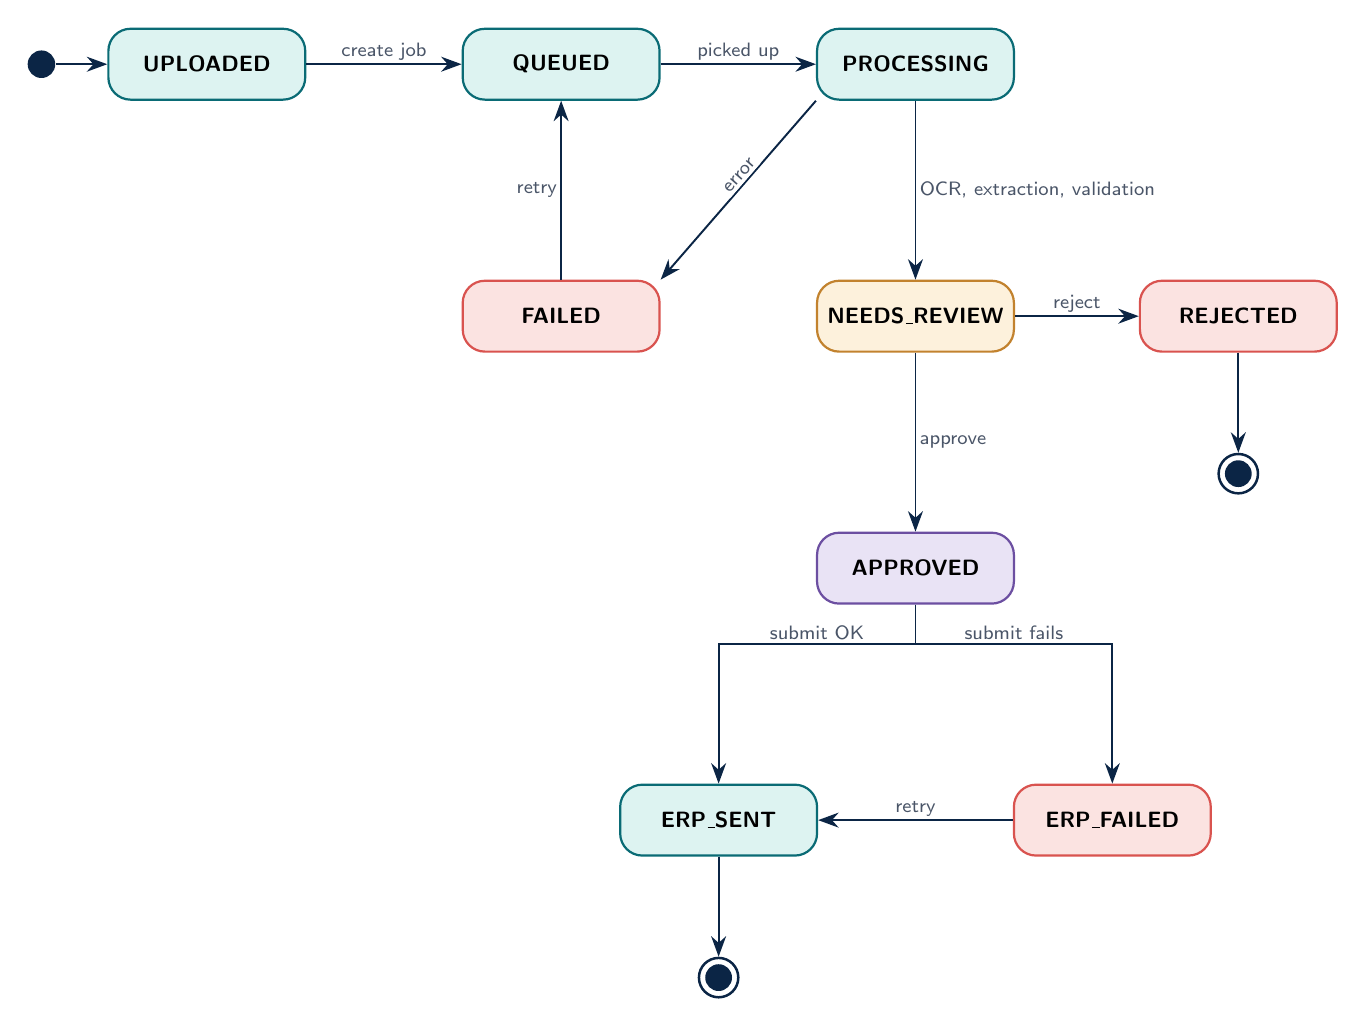
\begin{tikzpicture}[x=1cm,y=1cm]
\node[initial] (i) at (-0.6,0) {};
\node[state] (up) at (1.5,0) {UPLOADED};
\node[state] (qu) at (6.0,0) {QUEUED};
\node[state] (pr) at (10.5,0) {PROCESSING};
\node[stateC] (fa) at (6.0,-3.2) {FAILED};
\node[stateA] (nr) at (10.5,-3.2) {NEEDS\_REVIEW};
\node[stateC] (rj) at (14.6,-3.2) {REJECTED};
\node[stateV] (ap) at (10.5,-6.4) {APPROVED};
\node[state] (es) at (8.0,-9.6) {ERP\_SENT};
\node[stateC] (ef) at (13.0,-9.6) {ERP\_FAILED};
\node[final] (f) at (8.0,-11.6) {};
\node[final] (f2) at (14.6,-5.2) {};
\draw[arr] (i) -- (up);
\draw[arr] (up) -- node[lbl,above]{create job} (qu);
\draw[arr] (qu) -- node[lbl,above]{picked up} (pr);
\draw[arr] (pr) -- node[lbl,right]{OCR, extraction, validation} (nr);
\draw[arr] (pr.south west) -- node[lbl,above,sloped,pos=0.45]{error} (fa.north east);
\draw[arr] (fa) -- node[lbl,left]{retry} (qu);
\draw[arr] (nr) -- node[lbl,above]{reject} (rj);
\draw[arr] (rj) -- (f2);
\draw[arr] (nr) -- node[lbl,right]{approve} (ap);
\draw[arr] (ap.south) -- ++(0,-0.5) -| node[lbl,pos=0.25,above]{submit OK} (es.north);
\draw[arr] (ap.south) -- ++(0,-0.5) -| node[lbl,pos=0.25,above]{submit fails} (ef.north);
\draw[arr] (ef) -- node[lbl,above]{retry} (es);
\draw[arr] (es) -- (f);
\end{tikzpicture}
}
\caption{Document lifecycle. The filled dot is the start; double circles are end states that can still be left only by an explicit retry or reprocess action.}\label{fig:p2state}
\end{figure}

\begin{figure}[H]\centering
\resizebox{0.95\textwidth}{!}{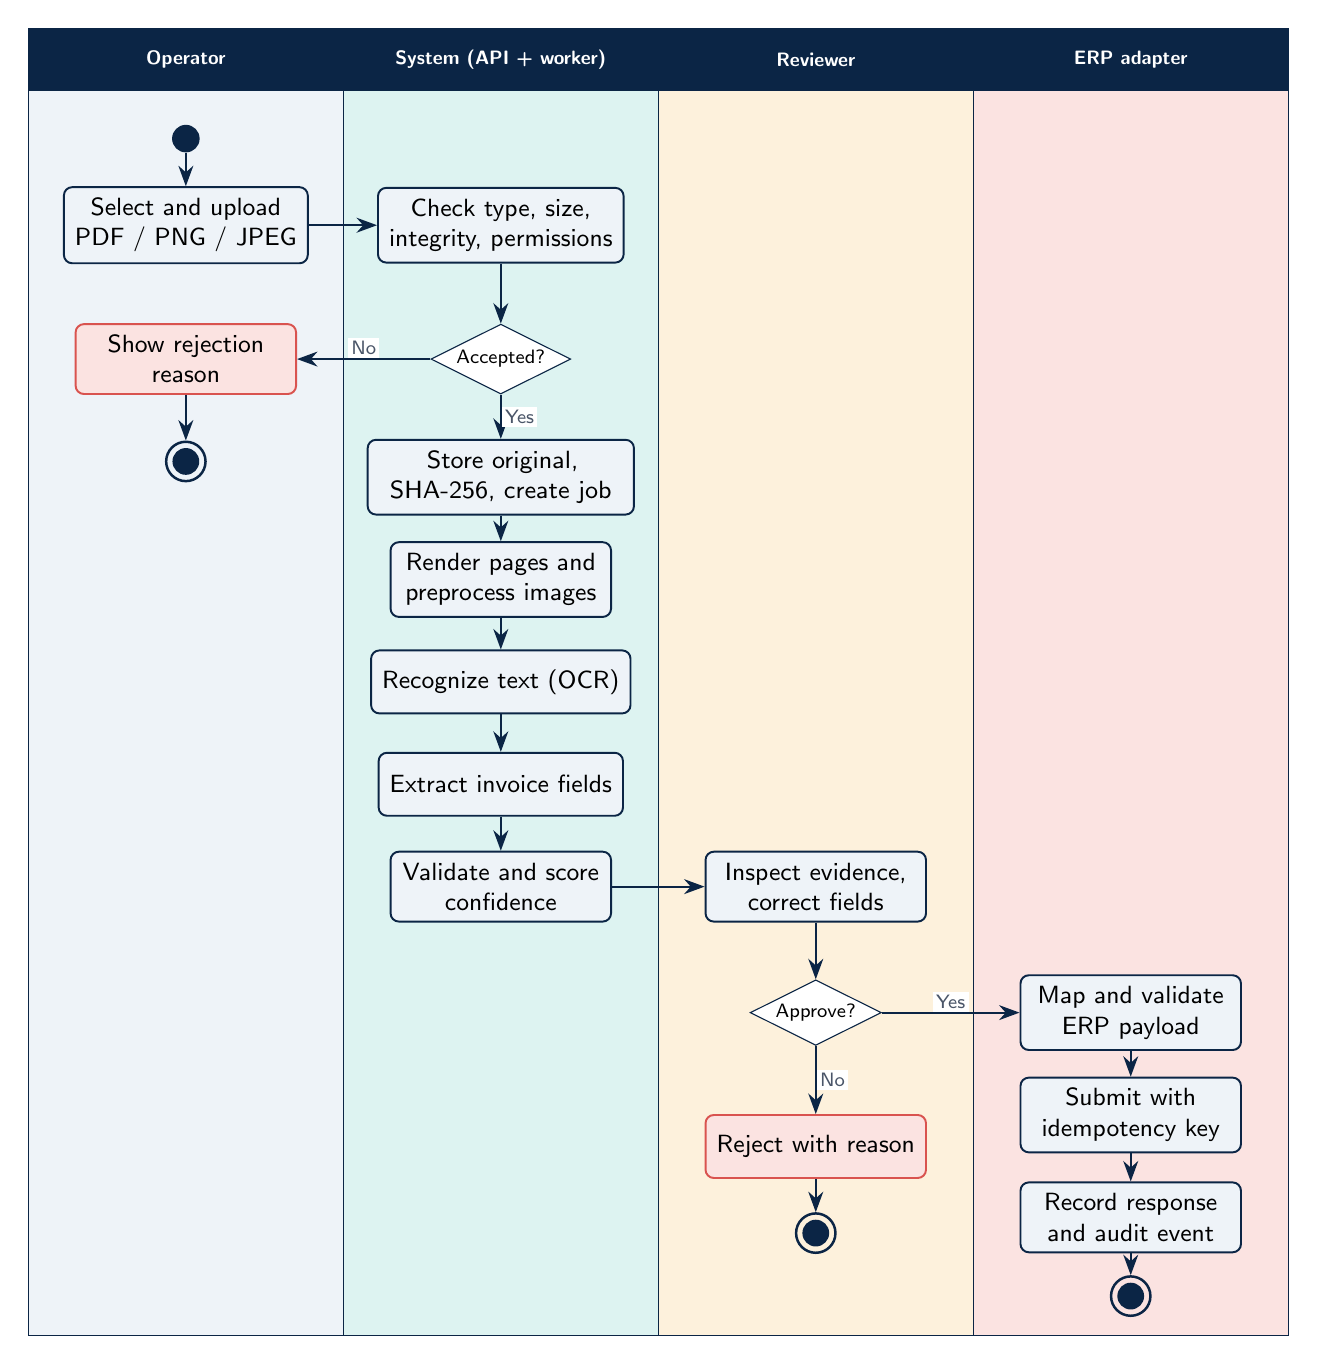
\begin{tikzpicture}[x=1cm,y=1cm]
% lanes
\foreach \x/\t/\c in {0/Operator/mist, 4/System (API + worker)/mint, 8/Reviewer/sand, 12/ERP adapter/blush}{
  \fill[\c] (\x,-16.4) rectangle (\x+4,0.2);
  \draw[navy,line width=0.5pt] (\x,-16.4) rectangle (\x+4,0.2);
  \fill[navy] (\x,-0.6) rectangle (\x+4,0.2);
  \node[text=white,font=\sffamily\bfseries\scriptsize] at (\x+2,-0.2) {\t};}
% nodes
\node[initial] (s) at (2,-1.2) {};
\node[box,minimum width=2.8cm] (a1) at (2,-2.3) {Select and upload\\ PDF / PNG / JPEG};
\node[box,minimum width=2.8cm] (a2) at (6,-2.3) {Check type, size,\\ integrity, permissions};
\node[diamond,aspect=2,draw=navy,fill=white,inner sep=1pt,font=\sffamily\scriptsize,align=center] (d1) at (6,-4.0) {Accepted?};
\node[box,minimum width=2.8cm,fill=blush,draw=coral] (a3) at (2,-4.0) {Show rejection\\ reason};
\node[final] (e1) at (2,-5.3) {};
\node[box,minimum width=2.8cm,text width=3.1cm] (a4) at (6,-5.5) {Store original, SHA-256, create job};
\node[box,minimum width=2.8cm] (a5) at (6,-6.8) {Render pages and\\ preprocess images};
\node[box,minimum width=2.8cm] (a6) at (6,-8.1) {Recognize text (OCR)};
\node[box,minimum width=2.8cm] (a7) at (6,-9.4) {Extract invoice fields};
\node[box,minimum width=2.8cm] (a8) at (6,-10.7) {Validate and score\\ confidence};
\node[box,minimum width=2.8cm] (b1) at (10,-10.7) {Inspect evidence,\\ correct fields};
\node[diamond,aspect=2,draw=navy,fill=white,inner sep=1pt,font=\sffamily\scriptsize,align=center] (d2) at (10,-12.3) {Approve?};
\node[box,minimum width=2.8cm,fill=blush,draw=coral] (b2) at (10,-14.0) {Reject with reason};
\node[final] (e2) at (10,-15.1) {};
\node[box,minimum width=2.8cm] (c1) at (14,-12.3) {Map and validate\\ ERP payload};
\node[box,minimum width=2.8cm] (c2) at (14,-13.6) {Submit with\\ idempotency key};
\node[box,minimum width=2.8cm] (c3) at (14,-14.9) {Record response\\ and audit event};
\node[final] (e3) at (14,-15.9) {};
% edges
\draw[arr] (s) -- (a1);
\draw[arr] (a1) -- (a2.west);
\draw[arr] (a2) -- (d1);
\draw[arr] (d1.west) -- node[lbl,above]{No} (a3.east);
\draw[arr] (a3) -- (e1);
\draw[arr] (d1) -- node[lbl,right]{Yes} (a4);
\foreach \a/\b in {a4/a5,a5/a6,a6/a7,a7/a8}{\draw[arr] (\a) -- (\b);}
\draw[arr] (a8) -- (b1);
\draw[arr] (b1) -- (d2);
\draw[arr] (d2) -- node[lbl,right]{No} (b2);
\draw[arr] (b2) -- (e2);
\draw[arr] (d2.east) -- node[lbl,above]{Yes} (c1.west);
\draw[arr] (c1) -- (c2);
\draw[arr] (c2) -- (c3);
\draw[arr] (c3) -- (e3);
\end{tikzpicture}
}
\caption{Activity view of the whole flow, including the review decision and the ERP result.}\label{fig:p2activity}
\end{figure}

\section{Stage by stage}
{\tblstart\footnotesize
\begin{longtable}{L{2.3cm}L{4.3cm}L{3.3cm}L{1.9cm}L{2.2cm}}
\hdrrow \hdr{Stage} & \hdr{What happens} & \hdr{Writes} & \hdr{Status after} & \hdr{On failure}\\ \endhead
1. Receive and validate & Check type, content, size, pages and integrity (Section~\ref{sec:p2upload}). & Nothing yet if refused. & --- & Refuse with 400, 413 or 415.\\
2. Store & Save the original in protected storage under an opaque key; compute SHA-256. & \texttt{documents} row; audit event UPLOAD. & UPLOADED & Delete the partial file; return 500.\\
3. Queue & Mark ready for the worker; return \texttt{202} with the document ID. & Status. & QUEUED & Stays QUEUED; the worker picks it up later.\\
4. Preprocess & Render PDF pages to images; deskew, denoise, normalise contrast; segment lines. & \texttt{processing\_runs} row; page images in storage. & PROCESSING & Category UNREADABLE or TIMEOUT.\\
5. Recognise & Run the selected OCR engine; keep text, line boxes and confidence. & Run engine and model version. & PROCESSING & Category OCR\_ERROR.\\
6. Extract & Map recognised text to the invoice fields and line items; keep page and box. & \texttt{extracted\_fields}, \texttt{extracted\_line\_items}. & PROCESSING & Fields left empty and flagged, not invented.\\
7. Validate & Apply the rules of Section~\ref{sec:p2rules}; compute findings and a validation status per field. & \texttt{validation\_findings}. & PROCESSING & Rule error is logged; record still goes to review.\\
8. Route & Always send to human review in the prototype. & Run status SUCCEEDED. & NEEDS\_REVIEW & Unrecoverable error: FAILED.\\
9. Review & Reviewer corrects fields with a reason, then approves or rejects. & \texttt{field\_corrections}, \texttt{reviews}, audit. & APPROVED or REJECTED & ---\\
10. Submit & Build the ERP payload; send with the idempotency key; record the result. & \texttt{erp\_attempts}, audit. & ERP\_SENT or ERP\_FAILED & Retry is safe (Chapter~\ref{ch:p2sec}).\\
\hline
\end{longtable}}

\section{File validation at upload}\label{sec:p2upload}
{\tblstart\small
\begin{longtable}{L{3.2cm}L{6.6cm}L{4.0cm}}
\hdrrow \hdr{Check} & \hdr{Rule} & \hdr{Response}\\ \endhead
Empty file & Size must be above zero. & 400 \texttt{VALIDATION\_ERROR}\\
File type & Extension is \texttt{.pdf}, \texttt{.png}, \texttt{.jpg} or \texttt{.jpeg}, and the first bytes of the content match PDF, PNG or JPEG. The client-supplied MIME type is not trusted on its own. & 415 \texttt{UNSUPPORTED\_MEDIA\_TYPE}\\
Size & At most \texttt{max\_upload\_bytes} (10 MB at the start). & 413 \texttt{FILE\_TOO\_LARGE}\\
Pages & PDF has at most \texttt{max\_pdf\_pages} pages (10 at the start). & 400 \texttt{VALIDATION\_ERROR}\\
Integrity & The file opens with the PDF or image library. & 400 \texttt{VALIDATION\_ERROR}\\
Duplicate file & Same SHA-256 as an earlier document: accepted, then reported as an information finding so a person decides. & 202 with a warning\\
\hline
\end{longtable}}

\section{Validation rules}\label{sec:p2rules}
{\tblstart\small
\begin{longtable}{L{3.0cm}L{6.2cm}L{1.8cm}L{2.8cm}}
\hdrrow \hdr{Rule code} & \hdr{Check} & \hdr{Severity} & \hdr{Setting}\\ \endhead
REQUIRED\_FIELD & Supplier, invoice number, invoice date, subtotal, tax, total and currency are present and parse. & BLOCKING & ---\\
DATE & Dates parse; due date is not before invoice date; date is in a plausible range. & WARNING & ---\\
ARITHMETIC & Subtotal plus tax equals total within the tolerance. Never corrected automatically. & WARNING & \texttt{arithmetic\_\allowbreak tolerance}\\
CURRENCY & Currency code or symbol is known and consistent across fields. & WARNING & ---\\
DUPLICATE & Same supplier, invoice number, date and amount as an earlier approved or sent document. & WARNING & ---\\
ERP\_SCHEMA & The approved values satisfy the ERP payload schema. & BLOCKING & ---\\
\hline
\end{longtable}}
A BLOCKING finding prevents approval until the reviewer corrects the cause. A WARNING does not block, but the approval event stores which warnings were open, so the audit trail shows the reviewer saw them.

\section{Confidence and review routing}
Confidence is a signal for the reviewer, not proof of correctness. The two thresholds live in \texttt{system\_settings} and the starting values (0.90 and 0.70) are \textbf{provisional}. They must be chosen on validation data after the OCR baseline exists, never on the test set.
{\tblstart\small
\begin{longtable}{L{5.2cm}L{4.4cm}L{4.2cm}}
\hdrrow \hdr{Condition on a field} & \hdr{Shown to the reviewer as} & \hdr{Reviewer action}\\ \endhead
Confidence at or above \texttt{confidence\_accept} and no failed rule & Accepted (green, with a text label). & May confirm without changes.\\
Between \texttt{confidence\_review} and \texttt{confidence\_accept} & Highlighted (amber, REVIEW). & Should check against the source.\\
Below \texttt{confidence\_review}, or a failed rule & Needs attention (red, REVIEW or FAIL). & Must confirm or correct before approval.\\
\hline
\end{longtable}}
In the prototype every document goes to review, whatever the confidence (rule BR-1). A later version could skip review for very high confidence, but only after measured error rates justify it.

\section{Failure and retry}
{\tblstart\small
\begin{longtable}{L{3.0cm}L{4.4cm}L{6.4cm}}
\hdrrow \hdr{Error category} & \hdr{Kind} & \hdr{Behaviour (values provisional)}\\ \endhead
UNREADABLE & Permanent & Run FAILED, document FAILED. A person uploads a better file or requests reprocessing.\\
OCR\_ERROR & Possibly temporary & Up to two automatic retries, then FAILED.\\
TIMEOUT & Temporary & Up to two automatic retries with a longer limit, then FAILED.\\
STORAGE\_ERROR & Temporary & Retry; if it keeps failing, FAILED and an alert in the log.\\
INTERNAL & Unknown & FAILED; details only in the server log, not in the response.\\
\hline
\end{longtable}}
\texttt{documents.retry\_count} records automatic retries. A manual reprocess from FAILED or REJECTED creates a new run and returns the document to QUEUED; the earlier runs stay.

\section{Upload sequence}
\begin{figure}[H]\centering
\resizebox{0.95\textwidth}{!}{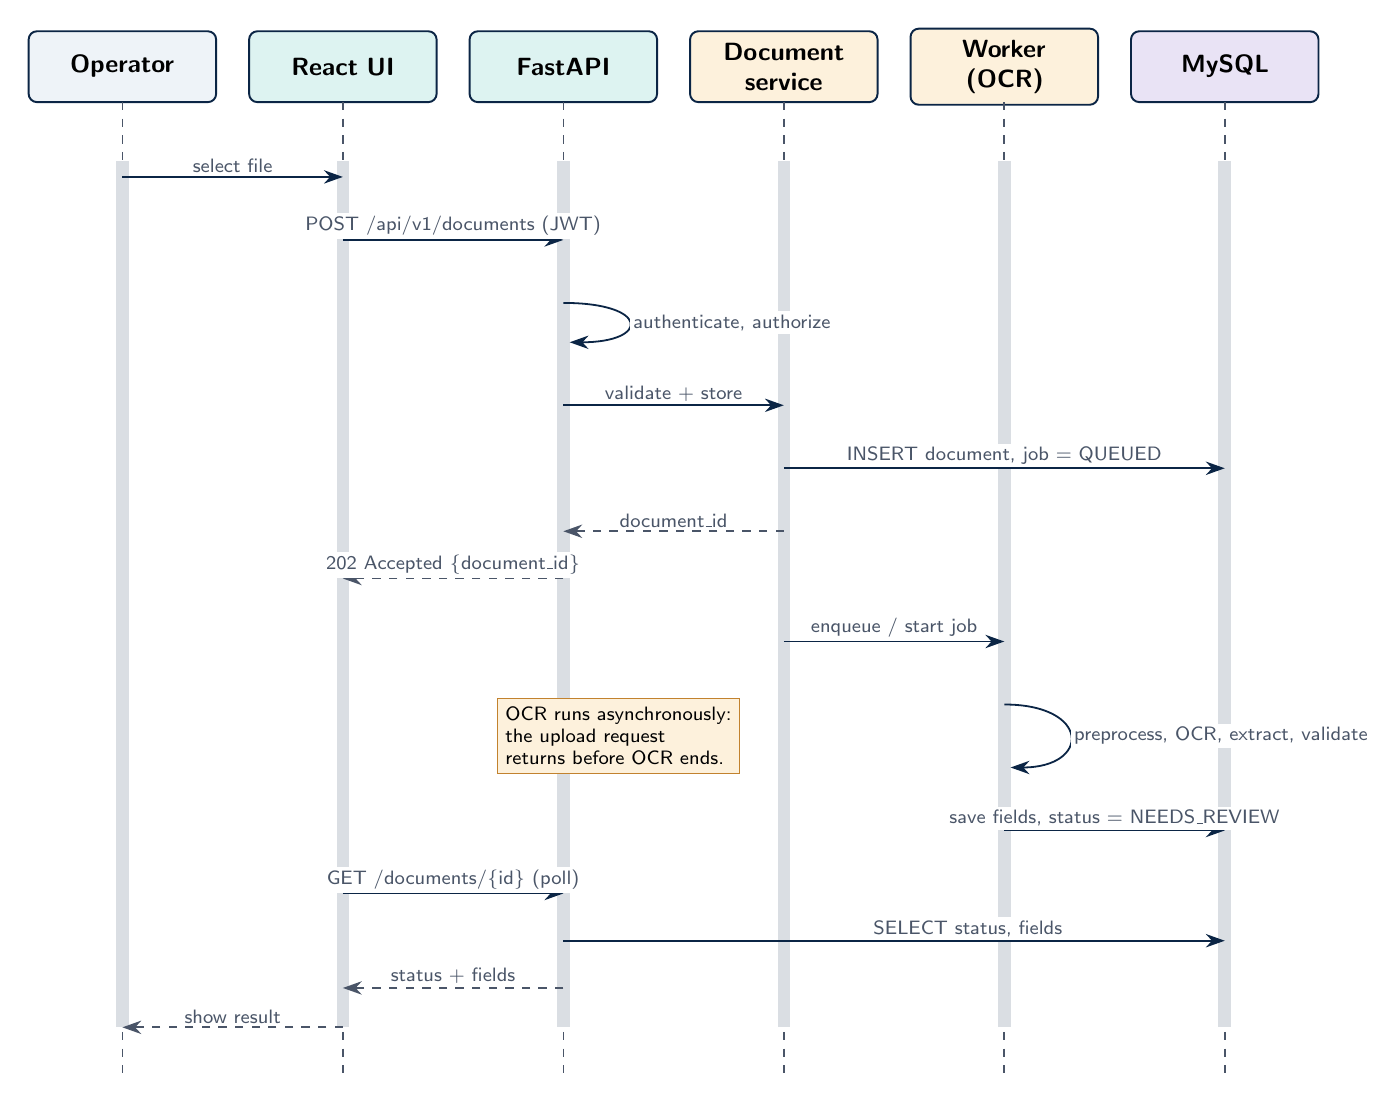
\begin{tikzpicture}[x=1cm,y=1cm]
\def\ys{-0.9}
\foreach \x/\n/\c in {0.9/Operator/mist, 3.7/React UI/mint, 6.5/FastAPI/mint, 9.3/Document\\service/sand, 12.1/Worker\\(OCR)/sand, 14.9/MySQL/lilac}{
  \node[box,fill=\c,minimum width=2.3cm,text width=2.1cm,minimum height=0.9cm] (p\x) at (\x,0) {\textbf{\n}};
  \draw[lifeline] (\x,-0.45) -- (\x,-12.8);
  \fill[navy!15] (\x-0.08,-1.2) rectangle (\x+0.08,-12.2);}
% messages (y descending)
\draw[msg] (0.9,-1.4) -- node[lbl,above]{select file} (3.7,-1.4);
\draw[msg] (3.7,-2.2) -- node[lbl,above]{POST /api/v1/documents (JWT)} (6.5,-2.2);
\draw[msg] (6.5,-3.0) .. controls (7.6,-3.0) and (7.6,-3.5) .. node[lbl,right,pos=0.5]{authenticate, authorize} (6.58,-3.5);
\draw[msg] (6.5,-4.3) -- node[lbl,above]{validate + store} (9.3,-4.3);
\draw[msg] (9.3,-5.1) -- node[lbl,above]{INSERT document, job = QUEUED} (14.9,-5.1);
\draw[ret] (9.3,-5.9) -- node[lbl,above]{document\_id} (6.5,-5.9);
\draw[ret] (6.5,-6.5) -- node[lbl,above]{202 Accepted \{document\_id\}} (3.7,-6.5);
\draw[msg] (9.3,-7.3) -- node[lbl,above]{enqueue / start job} (12.1,-7.3);
\draw[msg] (12.1,-8.1) .. controls (13.2,-8.1) and (13.2,-8.9) .. node[lbl,right,pos=0.5]{preprocess, OCR, extract, validate} (12.18,-8.9);
\draw[msg] (12.1,-9.7) -- node[lbl,above]{save fields, status = NEEDS\_REVIEW} (14.9,-9.7);
\draw[msg] (3.7,-10.5) -- node[lbl,above]{GET /documents/\{id\} (poll)} (6.5,-10.5);
\draw[msg] (6.5,-11.1) .. controls (10.7,-11.1) and (13.2,-11.1) .. node[lbl,above,pos=0.5]{SELECT status, fields} (14.9,-11.1);
\draw[ret] (6.5,-11.7) -- node[lbl,above]{status + fields} (3.7,-11.7);
\draw[ret] (3.7,-12.2) -- node[lbl,above]{show result} (0.9,-12.2);
% async note
\node[draw=amber!80!black,fill=sand,font=\sffamily\scriptsize,align=left,inner sep=3pt] at (7.2,-8.5) {OCR runs asynchronously:\\ the upload request\\ returns before OCR ends.};
\end{tikzpicture}
}
\caption{Upload and asynchronous processing. The user receives an identifier immediately and follows the status.}\label{fig:p2sequpload}
\end{figure}

% =====================================================================
\chapter{REST API Design}\label{ch:p2api}
\emph{Story US-09.} The chapter defines endpoints for uploading and retrieving documents, for extracted fields and review decisions, the response formats and error handling, and the authentication and authorisation rules. The complete contract is the file \texttt{openapi.yaml}.

\section{Conventions}
\begin{itemize}
\item Base path \texttt{/api/v1}; JSON bodies; \texttt{multipart/form-data} for uploads.
\item Names in \texttt{snake\_case}; identifiers are UUID strings; times are ISO 8601 in UTC.
\item Lists are paged with \texttt{page} (from 1) and \texttt{page\_size} (default 20, at most 100) and return \texttt{items}, \texttt{page}, \texttt{page\_size} and \texttt{total}.
\item Clients must ignore unknown response fields, so fields can be added without a new version. A breaking change would become \texttt{/api/v2}.
\item Every response carries a request identifier that also appears in the server log.
\end{itemize}

\section{Authentication and authorisation}
A user signs in with e-mail and password at \texttt{POST /auth/login} and receives a short-lived bearer token (the contract example uses 1800 seconds, a provisional value). Every other endpoint, except the two health checks, requires the token. The backend looks up the user and role on each request and refuses with \texttt{401} (no or invalid token) or \texttt{403} (role not allowed). Repeated failed logins lock the account for a short time and the login endpoint returns \texttt{429} when rate-limited.

{\tblstart\small
\begin{longtable}{L{6.2cm}C{1.8cm}C{1.8cm}C{1.8cm}}
\hdrrow \hdr{Function} & \hdr{Operator} & \hdr{Reviewer} & \hdr{Admin}\\ \endhead
Sign in, read own profile & yes & yes & yes\\
Upload; list and view own documents & yes & yes & yes\\
List and view \emph{all} documents; dashboard of all documents & --- & yes & yes\\
Request reprocessing & own & yes & yes\\
Read extracted fields; view source file and page images & --- & yes & yes\\
Correct fields; approve; reject & --- & yes & yes\\
Submit to ERP; view integration history; export & --- & yes & yes\\
View a document's audit trail & --- & yes & yes\\
Manage users; change settings & --- & --- & yes\\
\hline
\end{longtable}}
A document that a user may not see is reported as \texttt{404}, not \texttt{403}, so the API does not confirm that it exists.

\section{Endpoint catalogue}
The table is generated from \texttt{openapi.yaml}. \emph{Roles} abbreviates Operator (Op), Reviewer (Rev) and Administrator (Adm).
{\tblstart\footnotesize
\begin{longtable}{L{1.3cm}L{5.0cm}L{1.6cm}L{4.4cm}L{1.9cm}}
\hdrrow \hdr{Method} & \hdr{Path (after \texttt{/api/v1})} & \hdr{Roles} & \hdr{Purpose} & \hdr{Status codes}\\ \endhead
GET & \texttt{/\allowbreak health} & public & Liveness check \emph{(exists)} & 200\\
GET & \texttt{/\allowbreak health/\allowbreak db} & public & Database readiness check \emph{(exists)} & 200, 503\\
POST & \texttt{/\allowbreak auth/\allowbreak login} & public & Sign in and receive an access token & 200, 401, 429\\
GET & \texttt{/\allowbreak auth/\allowbreak me} & Op, Rev, Adm & Current user profile & 200, 401\\
POST & \texttt{/\allowbreak documents} & Op, Rev, Adm & Upload a document and create a processing job & 202, 400, 401, 413, 415\\
GET & \texttt{/\allowbreak documents} & Op, Rev, Adm & List and filter documents & 200, 401\\
GET & \texttt{/\allowbreak documents/\allowbreak \{document\_id\}} & Op, Rev, Adm & Document metadata, status and processing summary & 200, 401, 404\\
GET & \texttt{/\allowbreak documents/\allowbreak \{document\_id\}/\allowbreak result} & Rev, Adm & Extracted fields, line items and validation findings of the latest run & 200, 403, 404, 409\\
GET & \texttt{/\allowbreak documents/\allowbreak \{document\_id\}/\allowbreak file} & Rev, Adm & Download the original file after an authorisation check & 200, 403, 404\\
GET & \texttt{/\allowbreak documents/\allowbreak \{document\_id\}/\allowbreak pages/\allowbreak \{page\_no\}/\allowbreak image} & Rev, Adm & Rendered page image for the review screen & 200, 403, 404\\
PATCH & \texttt{/\allowbreak documents/\allowbreak \{document\_id\}/\allowbreak fields} & Rev, Adm & Save reviewer corrections (reason required, original value kept) & 200, 400, 403, 404, 409\\
POST & \texttt{/\allowbreak documents/\allowbreak \{document\_id\}/\allowbreak approve} & Rev, Adm & Approve the record (blocked while a BLOCKING finding is open) & 200, 403, 404, 409\\
POST & \texttt{/\allowbreak documents/\allowbreak \{document\_id\}/\allowbreak reject} & Rev, Adm & Reject the record with a reason & 200, 400, 403, 409\\
POST & \texttt{/\allowbreak documents/\allowbreak \{document\_id\}/\allowbreak reprocess} & Op, Rev, Adm & Start a new processing run for a FAILED or REJECTED document & 202, 403, 409\\
POST & \texttt{/\allowbreak documents/\allowbreak \{document\_id\}/\allowbreak submit} & Rev, Adm & Send an APPROVED record to the ERP adapter (idempotent) & 200, 403, 409, 502\\
GET & \texttt{/\allowbreak documents/\allowbreak \{document\_id\}/\allowbreak erp-attempts} & Rev, Adm & Integration history of one document & 200, 403, 404\\
GET & \texttt{/\allowbreak documents/\allowbreak \{document\_id\}/\allowbreak audit} & Rev, Adm & Audit trail of one document & 200, 403, 404\\
GET & \texttt{/\allowbreak dashboard/\allowbreak summary} & Op, Rev, Adm & Counts by status, review queue size and recent failures & 200\\
GET & \texttt{/\allowbreak exports/\allowbreak documents} & Rev, Adm & Export approved records as JSON or CSV & 200, 403\\
GET & \texttt{/\allowbreak users} & Adm & List users & 200, 403\\
POST & \texttt{/\allowbreak users} & Adm & Create a user & 201, 400, 403, 409\\
PATCH & \texttt{/\allowbreak users/\allowbreak \{user\_id\}} & Adm & Change role or deactivate a user & 200, 403, 404\\
GET & \texttt{/\allowbreak settings} & Adm & Read thresholds and validation settings & 200, 403\\
PUT & \texttt{/\allowbreak settings/\allowbreak \{setting\_key\}} & Adm & Change one setting (audited) & 200, 400, 403, 404\\
\hline
\end{longtable}}


\section{Examples}
\subsection{Sign in}
\begin{lstlisting}[language=Python,morekeywords={true,false,null}]
POST /api/v1/auth/login
{ "email": "reviewer@example.org", "password": "********" }

200 OK
{ "access_token": "<jwt>", "token_type": "bearer", "expires_in": 1800,
  "user": { "user_id": "7c1f...", "email": "reviewer@example.org",
            "full_name": "A. Reviewer", "role": "REVIEWER", "is_active": true } }
\end{lstlisting}

\subsection{Upload}
\begin{lstlisting}[language=Python,morekeywords={true,false,null}]
POST /api/v1/documents          (multipart, field "file")

202 Accepted
{ "document_id": "b3a9...", "original_filename": "INV-2026-001.pdf",
  "status": "QUEUED", "created_at": "2026-10-16T08:12:03Z" }
\end{lstlisting}

\subsection{Extraction result}
\begin{lstlisting}[language=Python,morekeywords={true,false,null}]
GET /api/v1/documents/b3a9.../result

200 OK
{ "document_id": "b3a9...", "status": "NEEDS_REVIEW", "run_id": "55d0...",
  "review_required": true,
  "fields": [
    { "name": "invoice_number", "raw_value": "INV-2026-001", "value": "INV-2026-001",
      "confidence": 0.91, "validation": "PASS", "message": null, "page": 1,
      "bbox": { "x": 0.61, "y": 0.08, "w": 0.22, "h": 0.03 } },
    { "name": "total_amount", "raw_value": "125 000", "value": "125000.00",
      "confidence": 0.68, "validation": "REVIEW",
      "message": "Subtotal + tax does not equal total", "page": 1, "bbox": null } ],
  "line_items": [],
  "findings": [
    { "rule_code": "ARITHMETIC", "severity": "WARNING",
      "message": "Subtotal + tax differs from total by 3.00",
      "field_names": ["subtotal", "tax_amount", "total_amount"] } ] }
\end{lstlisting}
The values are synthetic examples that show the format; they are not output of an implemented endpoint.

\subsection{Correction}
\begin{lstlisting}[language=Python,morekeywords={true,false,null}]
PATCH /api/v1/documents/b3a9.../fields
{ "corrections": [
    { "name": "total_amount", "new_value": "125003.00",
      "reason": "Digit misread; total printed as 125 003" } ] }
\end{lstlisting}
The service stores the old value, the new value, the reason, the user and the time in \texttt{field\_corrections}, updates \texttt{reviewed\_value}, re-runs the validation rules for the document and returns the new result.

\section{Error model}
Every error has the same shape, so the frontend needs one error handler.
\begin{lstlisting}[language=Python,morekeywords={true,false,null}]
409 Conflict
{ "error": { "code": "INVALID_STATE",
             "message": "Document must be APPROVED before submission",
             "details": [], "request_id": "req_9f2c" } }
\end{lstlisting}
{\tblstart\small
\begin{longtable}{L{1.3cm}L{4.4cm}L{8.1cm}}
\hdrrow \hdr{HTTP} & \hdr{\texttt{error.code}} & \hdr{When}\\ \endhead
400 & VALIDATION\_ERROR & Malformed body, missing field, bad value, corrupt file, too many pages. \texttt{details} lists each field and issue.\\
401 & UNAUTHENTICATED & Missing, invalid or expired token; wrong password.\\
403 & FORBIDDEN & The role may not perform the action.\\
404 & NOT\_FOUND & No such resource, or the user may not see it.\\
409 & INVALID\_STATE & The status does not allow the action (for example approve while PROCESSING), or a blocking finding is open, or a user already exists.\\
413 & FILE\_TOO\_LARGE & Upload above the size limit.\\
415 & UNSUPPORTED\_MEDIA\_TYPE & File type not accepted.\\
429 & RATE\_LIMITED & Too many sign-in attempts.\\
502 & ERP\_UNAVAILABLE & The ERP rejected the record or could not be reached. The attempt is stored and retry is safe.\\
500 & INTERNAL\_ERROR & Unexpected error. The message is generic; details are only in the server log.\\
\hline
\end{longtable}}
Responses never contain stack traces, file-system paths, credentials or the internals of the ERP.

\section{Idempotency and concurrency}
\begin{itemize}
\item \texttt{POST /documents/\{id\}/submit} is safe to repeat. The key sent to the ERP is derived from the document identifier, so every retry uses the same key. If the document is already \texttt{ERP\_SENT}, the call returns the successful attempt and sends nothing.
\item Approve, reject and submit run in one transaction that locks the document row. Two reviewers acting at the same moment cannot both succeed: the second receives \texttt{409}.
\item The double-click problem in the interface is handled twice: the button is disabled after the first click, and the backend is idempotent anyway.
\end{itemize}

\section{How the contract will be used}
The contract is the shared reference for the React client and the FastAPI routers. When the routers are implemented, the schema FastAPI generates itself is compared with \texttt{openapi.yaml}, and differences are resolved deliberately, either by fixing the code or by revising the contract. A contract test for each endpoint is part of the Phase 3 and later work.

\chapter{User Interface Design}\label{ch:p2ui}
\emph{Story US-10.} The chapter sketches the dashboard, the upload page and the extraction-results and review screens, and defines the loading, success and error states.

\section{Users and tasks}
{\tblstart\small
\begin{longtable}{L{2.6cm}L{11.2cm}}
\hdrrow \hdr{User} & \hdr{Main tasks on screen}\\ \endhead
Operator & Upload invoices, see whether each one was accepted, follow its status, request reprocessing of a failed file.\\
Reviewer & Work through the review queue: compare the source page with the extracted values, correct, approve or reject, then submit to the ERP and check the result.\\
Administrator & Create users and set roles, adjust thresholds and limits, read the audit trail.\\
\hline
\end{longtable}}

\section{Screen map}
\begin{figure}[H]\centering
\resizebox{\textwidth}{!}{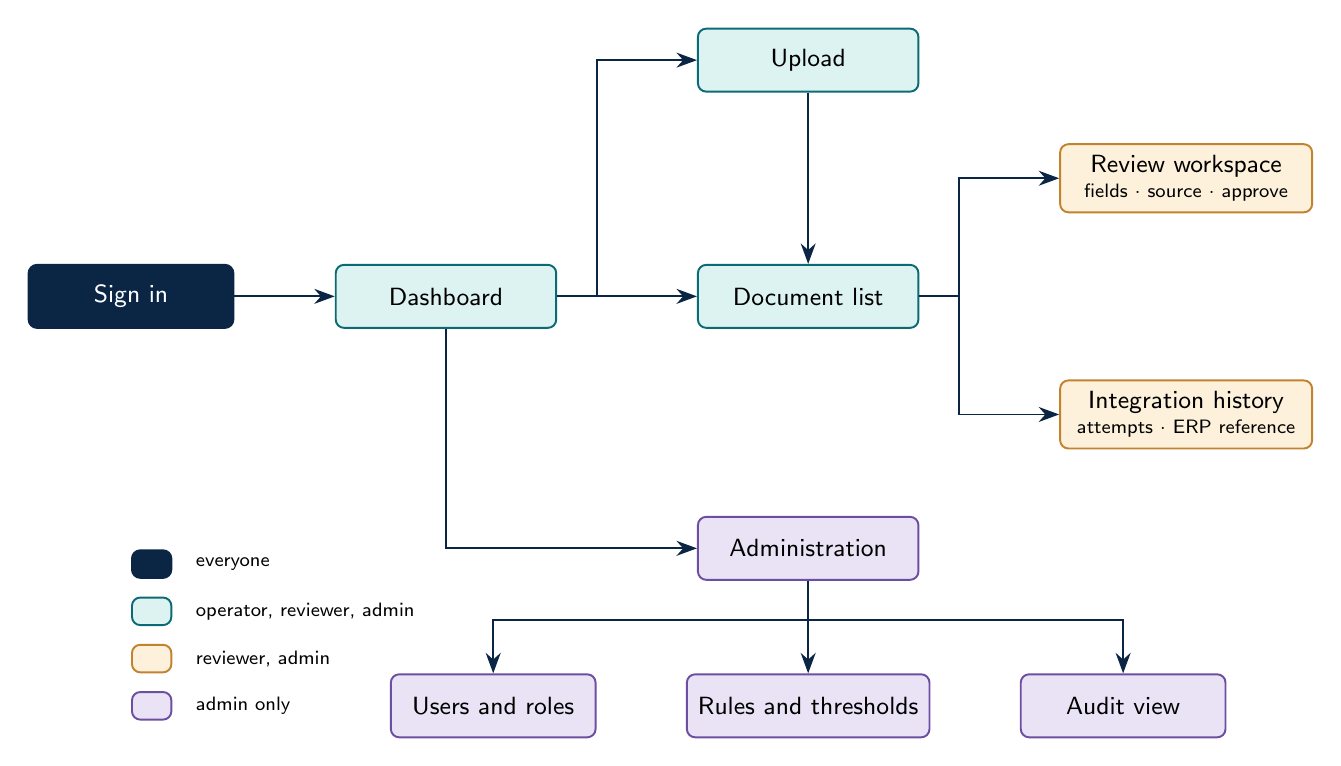
\begin{tikzpicture}[x=1cm,y=1cm]
\node[boxN,minimum width=2.6cm] (login) at (0,0) {Sign in};
\node[boxT,minimum width=2.8cm] (dash) at (4.0,0) {Dashboard};
\node[boxT,minimum width=2.8cm] (up) at (8.6,3.0) {Upload};
\node[boxT,minimum width=2.8cm] (list) at (8.6,0) {Document list};
\node[boxA,minimum width=3.2cm] (rev) at (13.4,1.5) {Review workspace\\[-2pt]\scriptsize fields $\cdot$ source $\cdot$ approve};
\node[boxA,minimum width=3.2cm] (hist) at (13.4,-1.5) {Integration history\\[-2pt]\scriptsize attempts $\cdot$ ERP reference};
\node[boxV,minimum width=2.8cm] (adm) at (8.6,-3.2) {Administration};
\node[boxV,minimum width=2.6cm] (usr) at (4.6,-5.2) {Users and roles};
\node[boxV,minimum width=3.0cm] (set) at (8.6,-5.2) {Rules and thresholds};
\node[boxV,minimum width=2.6cm] (aud) at (12.6,-5.2) {Audit view};
\draw[arr] (login) -- (dash);
\draw[arr] (dash.east) -- ++(0.5,0) |- (up.west);
\draw[arr] (dash) -- (list);
\draw[arr] (dash.south) -- ++(0,-1.2) |- (adm.west);
\draw[arr] (list.east) -- ++(0.5,0) |- (rev.west);
\draw[arr] (list.east) -- ++(0.5,0) |- (hist.west);
\draw[arr] (up.south) -- (list.north);
\draw[arr] (adm.south) -- ++(0,-0.5) -| (usr.north);
\draw[arr] (adm.south) -- (set.north);
\draw[arr] (adm.south) -- ++(0,-0.5) -| (aud.north);
% legend
\node[boxN,minimum width=0.5cm,minimum height=0.35cm,anchor=west] at (0,-3.4) {}; \node[font=\sffamily\scriptsize,anchor=west] at (0.7,-3.4) {everyone};
\node[boxT,minimum width=0.5cm,minimum height=0.35cm,anchor=west] at (0,-4.0) {}; \node[font=\sffamily\scriptsize,anchor=west] at (0.7,-4.0) {operator, reviewer, admin};
\node[boxA,minimum width=0.5cm,minimum height=0.35cm,anchor=west] at (0,-4.6) {}; \node[font=\sffamily\scriptsize,anchor=west] at (0.7,-4.6) {reviewer, admin};
\node[boxV,minimum width=0.5cm,minimum height=0.35cm,anchor=west] at (0,-5.2) {}; \node[font=\sffamily\scriptsize,anchor=west] at (0.7,-5.2) {admin only};
\end{tikzpicture}
}
\caption{Navigation map. Colour shows which roles may open a screen; the role is always checked again in the backend.}\label{fig:p2sitemap}
\end{figure}

\section{Dashboard}
The dashboard answers three questions at a glance: how much work is waiting, what failed, and what needs a person. The review queue is the main element and lists the oldest items first.
\begin{figure}[H]\centering
\resizebox{\textwidth}{!}{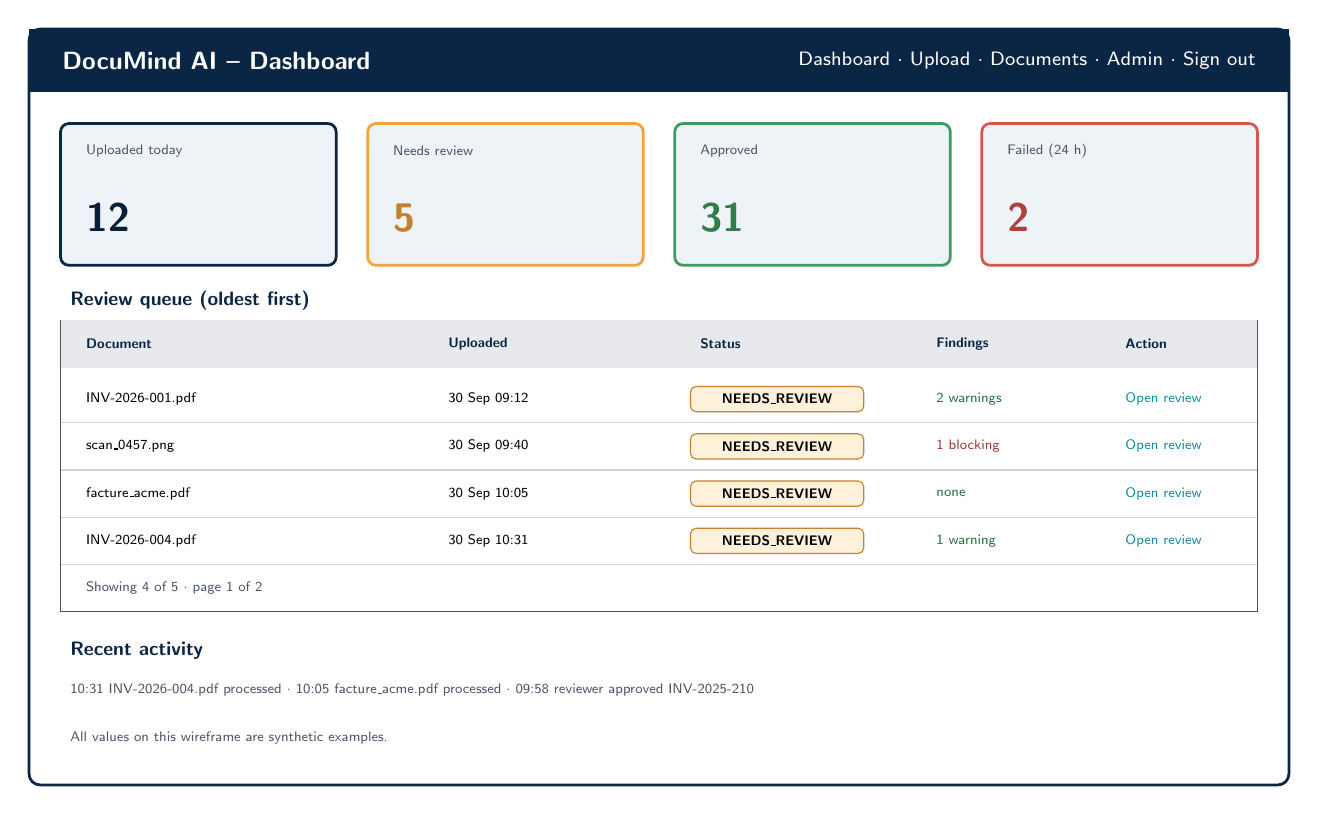
\begin{tikzpicture}[x=1cm,y=1cm]
\draw[rounded corners=4pt,fill=white,draw=navy,line width=1pt] (0,0) rectangle (16,9.6);
\fill[navy] (0,8.8) rectangle (16,9.6); \node[text=white,font=\sffamily\bfseries\small,anchor=west] at (0.3,9.2) {\projname{} -- Dashboard};
\node[text=white,font=\sffamily\scriptsize,anchor=east] at (15.7,9.2) {Dashboard $\cdot$ Upload $\cdot$ Documents $\cdot$ Admin $\cdot$ Sign out};
\foreach \x/\n/\v/\c in {0.4/Uploaded today/12/navy, 4.3/Needs review/5/amber, 8.2/Approved/31/leaf, 12.1/Failed (24 h)/2/coral}{
  \draw[rounded corners=3pt,fill=mist,draw=\c,line width=1pt] (\x,6.6) rectangle (\x+3.5,8.4);
  \node[font=\sffamily\tiny,text=slate,anchor=west] at (\x+0.2,8.05) {\n};
  \node[font=\sffamily\bfseries\Large,text=\c!80!black,anchor=west] at (\x+0.2,7.2) {\v};}
\node[font=\sffamily\scriptsize\bfseries,text=navy,anchor=west] at (0.4,6.15) {Review queue (oldest first)};
\draw[draw=slate,fill=white] (0.4,2.2) rectangle (15.6,5.9);
\fill[navy!10] (0.4,5.3) rectangle (15.6,5.9);
\foreach \x/\t in {0.6/Document, 5.2/Uploaded, 8.4/Status, 11.4/Findings, 13.8/Action}{\node[font=\sffamily\tiny\bfseries,anchor=west,text=navy] at (\x,5.6) {\t};}
\foreach \y/\a/\b/\c/\d in {4.9/INV-2026-001.pdf/30 Sep 09:12/2 warnings/leaf, 4.3/scan\_0457.png/30 Sep 09:40/1 blocking/coral, 3.7/facture\_acme.pdf/30 Sep 10:05/none/leaf, 3.1/INV-2026-004.pdf/30 Sep 10:31/1 warning/leaf}{
  \node[font=\sffamily\tiny,anchor=west] at (0.6,\y) {\a};
  \node[font=\sffamily\tiny,anchor=west] at (5.2,\y) {\b};
  \draw[rounded corners=2pt,fill=sand,draw=amber!80!black] (8.4,\y-0.16) rectangle (10.6,\y+0.16); \node[font=\sffamily\tiny\bfseries] at (9.5,\y) {NEEDS\_REVIEW};
  \node[font=\sffamily\tiny,anchor=west,text=\d!70!black] at (11.4,\y) {\c};
  \node[font=\sffamily\tiny,anchor=west,text=teal] at (13.8,\y) {Open review};
  \draw[slate!25] (0.4,\y-0.3) -- (15.6,\y-0.3);}
\node[font=\sffamily\tiny,text=slate,anchor=west] at (0.6,2.5) {Showing 4 of 5 $\cdot$ page 1 of 2};
\node[font=\sffamily\scriptsize\bfseries,text=navy,anchor=west] at (0.4,1.7) {Recent activity};
\node[font=\sffamily\tiny,text=slate,anchor=west] at (0.4,1.2) {10:31 INV-2026-004.pdf processed $\cdot$ 10:05 facture\_acme.pdf processed $\cdot$ 09:58 reviewer approved INV-2025-210};
\node[font=\sffamily\tiny,text=slate,anchor=west] at (0.4,0.6) {All values on this wireframe are synthetic examples.};
\end{tikzpicture}
}
\caption{Dashboard wireframe with synthetic values. Status is always shown as text as well as colour.}\label{fig:p2dash}
\end{figure}

\section{Upload page}
\begin{figure}[H]\centering
\resizebox{\textwidth}{!}{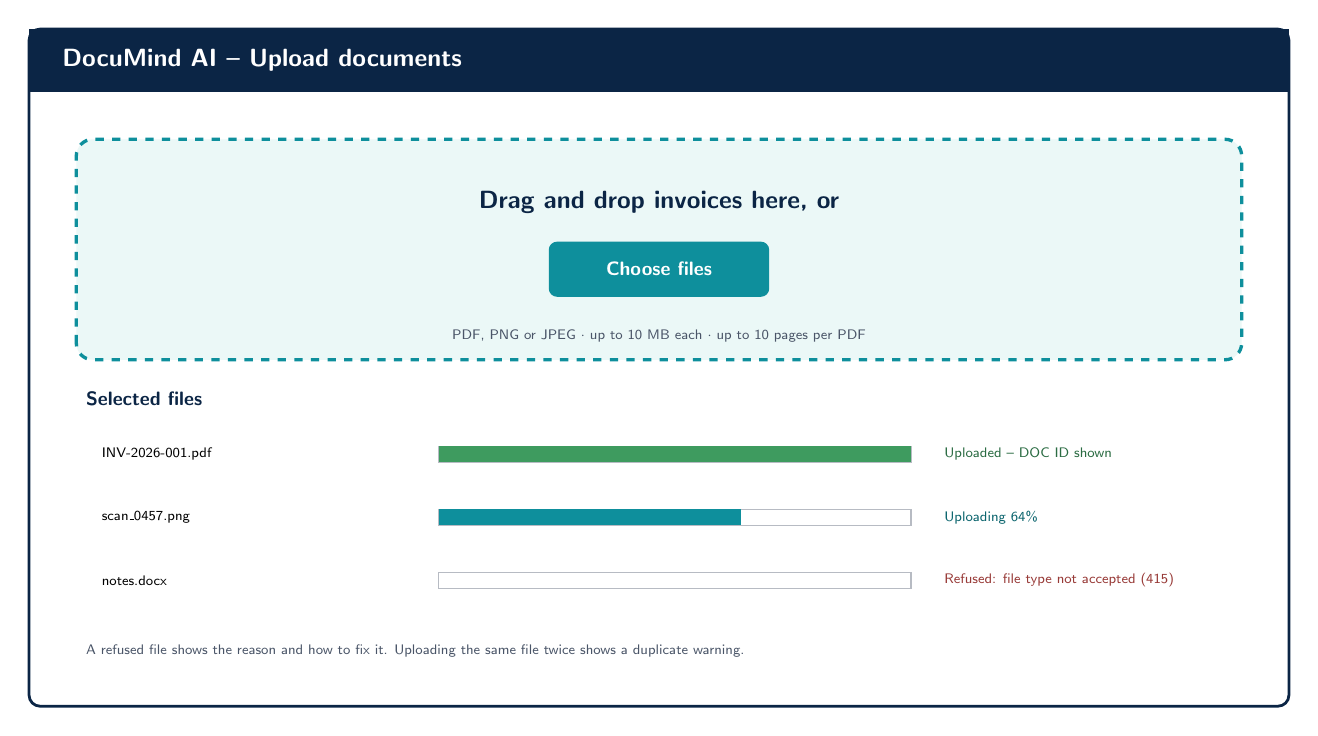
\begin{tikzpicture}[x=1cm,y=1cm]
\draw[rounded corners=4pt,fill=white,draw=navy,line width=1pt] (0,0) rectangle (16,8.6);
\fill[navy] (0,7.8) rectangle (16,8.6); \node[text=white,font=\sffamily\bfseries\small,anchor=west] at (0.3,8.2) {\projname{} -- Upload documents};
\draw[dashed,teal,line width=1.2pt,rounded corners=6pt,fill=mint!60] (0.6,4.4) rectangle (15.4,7.2);
\node[font=\sffamily\bfseries\small,text=navy] at (8,6.4) {Drag and drop invoices here, or};
\draw[rounded corners=3pt,fill=teal,draw=none] (6.6,5.2) rectangle (9.4,5.9); \node[text=white,font=\sffamily\bfseries\scriptsize] at (8,5.55) {Choose files};
\node[font=\sffamily\tiny,text=slate] at (8,4.7) {PDF, PNG or JPEG $\cdot$ up to 10 MB each $\cdot$ up to 10 pages per PDF};
\node[font=\sffamily\scriptsize\bfseries,text=navy,anchor=west] at (0.6,3.9) {Selected files};
\foreach \y/\n/\s/\p/\c in {3.2/INV-2026-001.pdf/Uploaded -- DOC ID shown/1.0/leaf, 2.4/scan\_0457.png/Uploading 64\%/0.64/teal, 1.6/notes.docx/Refused: file type not accepted (415)/0.0/coral}{
  \node[font=\sffamily\tiny,anchor=west] at (0.8,\y) {\n};
  \draw[slate!40,fill=white] (5.2,\y-0.1) rectangle (11.2,\y+0.1);
  \ifdim \p pt>0pt \fill[\c] (5.2,\y-0.1) rectangle ({5.2+6*\p},\y+0.1); \fi
  \node[font=\sffamily\tiny,anchor=west,text=\c!70!black] at (11.5,\y) {\s};}
\node[font=\sffamily\tiny,text=slate,anchor=west] at (0.6,0.7) {A refused file shows the reason and how to fix it. Uploading the same file twice shows a duplicate warning.};
\end{tikzpicture}
}
\caption{Upload wireframe showing a finished upload, one in progress and one refused file.}\label{fig:p2upload}
\end{figure}
The accepted formats and limits are shown before the user chooses a file, so refusals are rare, and a refused file states the reason and what to do.

\section{Extraction results and review}
The review workspace puts the source page on the left and the editable fields on the right. Selecting a field highlights its region on the page (FR-22). A field below the review threshold or with a failed rule is marked with the word REVIEW as well as a colour. Approve is disabled while a BLOCKING finding is open and explains why. Rejecting asks for a reason.
\begin{figure}[H]\centering
\resizebox{\textwidth}{!}{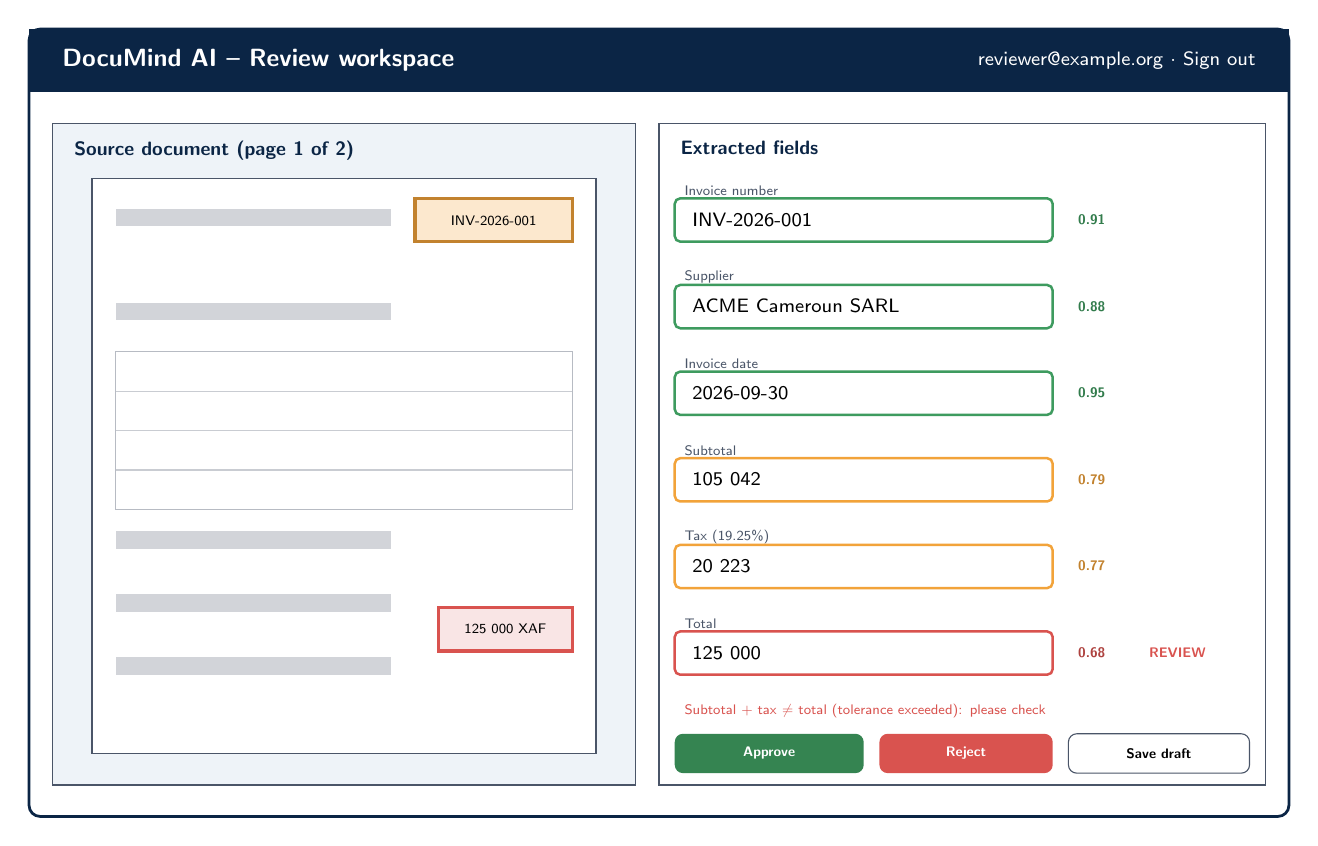
\begin{tikzpicture}[x=1cm,y=1cm]
\draw[rounded corners=4pt,fill=white,draw=navy,line width=1pt] (0,0) rectangle (16,10);
\fill[navy] (0,9.2) rectangle (16,10); \node[text=white,font=\sffamily\bfseries\small,anchor=west] at (0.3,9.6) {\projname{} -- Review workspace};
\node[text=white,font=\sffamily\scriptsize,anchor=east] at (15.7,9.6) {reviewer@example.org $\cdot$ Sign out};
\draw[fill=mist,draw=slate] (0.3,0.4) rectangle (7.7,8.8);
\node[font=\sffamily\scriptsize\bfseries,text=navy,anchor=north west] at (0.45,8.7) {Source document (page 1 of 2)};
\draw[fill=white,draw=slate] (0.8,0.8) rectangle (7.2,8.1);
\foreach \y in {7.5,6.3,3.4,2.6,1.8}{\fill[slate!25] (1.1,\y) rectangle (4.6,\y+0.22);}
\draw[amber!80!black,line width=1.2pt,fill=amber!25] (4.9,7.3) rectangle (6.9,7.85); \node[font=\sffamily\tiny] at (5.9,7.57) {INV-2026-001};
\draw[coral,line width=1.2pt,fill=coral!15] (5.2,2.1) rectangle (6.9,2.65); \node[font=\sffamily\tiny] at (6.05,2.38) {125 000 XAF};
\draw[slate!40] (1.1,5.9) rectangle (6.9,3.9); \foreach \y in {5.4,4.9,4.4}{\draw[slate!30] (1.1,\y) -- (6.9,\y);}
\draw[fill=white,draw=slate] (8.0,0.4) rectangle (15.7,8.8);
\node[font=\sffamily\scriptsize\bfseries,text=navy,anchor=north west] at (8.15,8.7) {Extracted fields};
\foreach \y/\n/\v/\cf/\col in {7.6/Invoice number/INV-2026-001/0.91/leaf, 6.5/Supplier/ACME Cameroun SARL/0.88/leaf, 5.4/Invoice date/2026-09-30/0.95/leaf, 4.3/Subtotal/105 042/0.79/amber, 3.2/Tax (19.25\%)/20 223/0.77/amber, 2.1/Total/125 000/0.68/coral}{
  \node[font=\sffamily\tiny,text=slate,anchor=west] at (8.2,\y+0.35) {\n};
  \draw[rounded corners=2pt,fill=white,draw=\col,line width=0.9pt] (8.2,\y-0.3) rectangle (13.0,\y+0.25);
  \node[font=\sffamily\scriptsize,anchor=west] at (8.3,\y-0.02) {\v};
  \node[font=\sffamily\tiny\bfseries,text=\col!80!black,anchor=west] at (13.2,\y-0.02) {\cf};}
\node[font=\sffamily\tiny\bfseries,text=coral,anchor=west] at (14.1,2.08) {REVIEW};
\node[font=\sffamily\tiny,text=coral,text width=6.8cm,anchor=north west] at (8.2,1.55) {Subtotal + tax $\neq$ total (tolerance exceeded): please check};
\draw[rounded corners=3pt,fill=leaf!85!black,draw=none] (8.2,0.55) rectangle (10.6,1.05); \node[text=white,font=\sffamily\bfseries\tiny] at (9.4,0.8) {Approve};
\draw[rounded corners=3pt,fill=coral,draw=none] (10.8,0.55) rectangle (13.0,1.05); \node[text=white,font=\sffamily\bfseries\tiny] at (11.9,0.8) {Reject};
\draw[rounded corners=3pt,fill=white,draw=slate] (13.2,0.55) rectangle (15.5,1.05); \node[font=\sffamily\bfseries\tiny] at (14.35,0.8) {Save draft};
\end{tikzpicture}
}
\caption{Review workspace wireframe (synthetic invoice).}\label{fig:p2review}
\end{figure}

\section{Other screens}
{\tblstart\small
\begin{longtable}{L{3.2cm}L{10.6cm}}
\hdrrow \hdr{Screen} & \hdr{Content}\\ \endhead
Sign in & E-mail and password; clear message for wrong credentials and for a locked account.\\
Document list & Search by ID, file name or invoice number; filter by status, type and date; paged table; link to detail.\\
Integration history & Attempts for one document: time, status, ERP reference, sanitised error, retry button when allowed.\\
Users and roles & Table of users, create form, role and active switch.\\
Rules and thresholds & The settings from \texttt{system\_settings} with description and last change; each change is audited.\\
Audit view & Filter by document, user and action; read-only.\\
\hline
\end{longtable}}

\section{Loading, success, empty and error states}
{\tblstart\footnotesize
\begin{longtable}{L{2.6cm}L{2.8cm}L{2.8cm}L{2.8cm}L{3.0cm}}
\hdrrow \hdr{Screen} & \hdr{Loading} & \hdr{Empty} & \hdr{Success} & \hdr{Error}\\ \endhead
Sign in & Button shows a spinner and is disabled. & --- & Go to dashboard. & Message under the form; no hint which of e-mail or password was wrong.\\
Dashboard & Placeholder tiles. & ``Nothing waiting'' message. & Counts and queue. & Banner with retry; page stays usable.\\
Upload & Progress bar per file. & Drop zone with instructions. & Document ID and status shown. & Reason and fix per file (413, 415, 400).\\
Document list & Skeleton rows. & ``No documents match'' with a clear-filters link. & Rows. & Banner with retry.\\
Review & Source and fields load independently. & Document not ready yet: show current status. & Toast ``Approved''. & Field-level messages; conflict (409) explains the current state.\\
Integration history & Skeleton rows. & ``Not submitted yet''. & Reference shown. & Sanitised error and retry.\\
Administration & Spinner on save. & No settings changed yet. & Toast ``Saved''. & Validation message next to the field.\\
\hline
\end{longtable}}

\section{Frontend structure and usability}
The React application is built with Vite. It keeps one API client module that adds the token, parses the error format of Chapter~\ref{ch:p2api} and exposes typed functions; screens never call the network directly. Server data is requested through a data-fetching layer (a library such as TanStack Query is proposed, to be confirmed in Phase 6). The application holds no database or ERP credentials. The token is kept in memory so that it is lost when the tab closes; whether to use a refresh mechanism is an open decision (Section~\ref{sec:p2open}).

Usability checks planned for the prototype: a keyboard-only pass through sign-in, upload and review; status never conveyed by colour alone; text contrast checked; and a short task test in which a reviewer finds and fixes a planted wrong value, as required by objective O7.

% =====================================================================
\chapter{Security and ERP Integration}\label{ch:p2sec}
\emph{Story US-11.} The chapter defines access permissions and credential management, file validation and data protection, the target Odoo version and available API, and validation and error handling before ERP submission.

\section{Threats and controls}
{\tblstart\footnotesize
\begin{longtable}{L{3.2cm}L{4.8cm}L{2.6cm}L{3.2cm}}
\hdrrow \hdr{Threat} & \hdr{Control} & \hdr{Enforced in} & \hdr{How it will be tested}\\ \endhead
Unauthorised access to documents & Bearer token, role check on every route, ownership check for operators, \texttt{404} for hidden items. & Backend & Test each role against each endpoint.\\
Password guessing & Password hashing, lockout counter, rate limit on login. & Backend & Repeated failed logins.\\
Malicious or corrupt upload & Type, content, size and page checks; files stored outside the web root under opaque keys; original filename never used as a path. & Backend, storage & Wrong-type, oversized and renamed files.\\
Path traversal or file disclosure & No path in any response; file served only after an authorisation check. & Backend & Request files without or with the wrong role.\\
Injection & Parameterised queries through the ORM; Pydantic validation of all input. & Backend & Hostile strings in every text field.\\
Tampering with history & Append-only audit table with triggers; corrections stored, never overwritten. & Database & Update and delete attempts (done, Section~\ref{sec:p2dbtests}).\\
Secret leakage & Secrets only in environment variables or a secret store; \texttt{.env} excluded from Git; tokens and passwords redacted from logs. & Deployment, backend & Repository and log review.\\
Cross-site calls & CORS limited to known origins (already implemented and tested). & Backend & Allowed and blocked origin tests.\\
Duplicate or lost ERP record & Idempotency key; transaction with row lock; stored attempts. & Backend, database & Retry and failure-injection tests.\\
Data exposure through logs or errors & Generic error messages; sanitised error text stored. & Backend & Force errors and inspect responses and logs.\\
\hline
\end{longtable}}

\section{Credentials and configuration}
\begin{itemize}
\item Database password, token signing key and ERP credentials are read from environment variables. The repository contains only \texttt{.env.example} with placeholders.
\item The ERP account is a dedicated integration user with only the rights needed to create vendor bills, and an API key rather than a personal password.
\item Credentials are different for development, demonstration and any later deployment, and can be rotated without code changes.
\item Passwords are stored with a slow, salted hash (Argon2id or bcrypt); the password is never logged.
\end{itemize}

\section{Data protection}
Invoices contain business and sometimes personal data. Access follows the role table of Chapter~\ref{ch:p2api}. Stored files are not publicly reachable. Transport uses HTTPS outside local development. Documents are not sent to external OCR or AI services. Backups of the database and the file store are taken together, and restoration is tested once. A retention period and a deletion procedure must be decided before real data is used.

\section{ERP integration}
\subsection{Target and options}
The target ERP is Odoo, reached through its external API and never by writing into its database. Odoo changes its external API between versions, so the version decides the implementation.
{\tblstart\small
\begin{longtable}{L{3.4cm}L{5.4cm}L{5.0cm}}
\hdrrow \hdr{Option} & \hdr{Reported situation} & \hdr{Use in this project}\\ \endhead
Mock ERP & Small service written for the project; same contract as the adapter. & First target; used for all automated tests.\\
XML-RPC / JSON-RPC & Reported as the most compatible choice for Odoo 14 to 18 and scheduled for removal in Odoo 20. & Implement if the available Odoo is version 18 or older.\\
JSON-2 API (bearer key, \texttt{/json/2/\allowbreak\{model\}/\allowbreak\{method\}}) & Reported as introduced in Odoo 19 as the replacement. & Implement if the available Odoo is version 19 or newer.\\
\hline
\end{longtable}}
\begin{warnbox}[Verify before implementing]
The statements in this table come from a third-party summary of the Odoo documentation (Apideck, ``How to integrate with the Odoo API''), not from the official page for a specific version, which could not be read during this phase. The exact endpoints, authentication and removal dates must be confirmed in the official documentation of the Odoo version that is actually available. This is open decision P2-D1.
\end{warnbox}

\subsection{Adapter interface}
The rest of the system sees only this interface. A mock, an XML-RPC and a JSON-2 adapter can implement it.
\begin{lstlisting}[language=Python]
class ErpAdapter(Protocol):
    name: str                                   # "MOCK" or "ODOO"
    def check_payload(self, record: ApprovedRecord) -> list[Finding]: ...
    def submit(self, record: ApprovedRecord, idempotency_key: str) -> ErpResult: ...

class ErpResult:
    ok: bool
    external_ref: str | None     # id of the created vendor bill
    error_category: str | None   # AUTH, VALIDATION, TIMEOUT, SERVER, DUPLICATE
    message: str | None          # sanitised
    http_status: int | None
\end{lstlisting}

\subsection{Field mapping}
The Phase 1 field list maps to a vendor bill. The Odoo names are candidates for a vendor bill (\texttt{account.move} with the vendor-bill type) and must be checked against the chosen version.
{\tblstart\small
\begin{longtable}{L{3.4cm}L{4.2cm}L{6.2cm}}
\hdrrow \hdr{Extracted field} & \hdr{Candidate Odoo field} & \hdr{Note}\\ \endhead
Supplier name, tax ID & Partner (\texttt{partner\_id}) & Find by tax ID or name; creating a new partner automatically is not done. If none matches, the reviewer chooses or the submission is blocked (ERP\_SCHEMA).\\
Invoice number & Vendor reference (\texttt{ref}) & Also used for the duplicate check on the ERP side.\\
Invoice date & Invoice date & ISO format.\\
Due date & Due date & Optional.\\
PO reference & Origin & Optional.\\
Line items & Invoice lines & Quantity, unit price and description per line; if no lines were extracted, one line with the subtotal is proposed and the reviewer confirms.\\
Subtotal, tax, total & Computed by the ERP from lines and taxes & Compared with the extracted values; a difference is a finding, not silently overridden.\\
Currency & Currency & Must exist in the ERP.\\
\hline
\end{longtable}}
Posting the bill (confirming it in accounting) is a separate ERP step. The prototype creates the bill in draft state so an accountant can post it; changing this is a decision for the ERP owner.

\subsection{Submission flow and idempotency}
\begin{figure}[H]\centering
\resizebox{0.95\textwidth}{!}{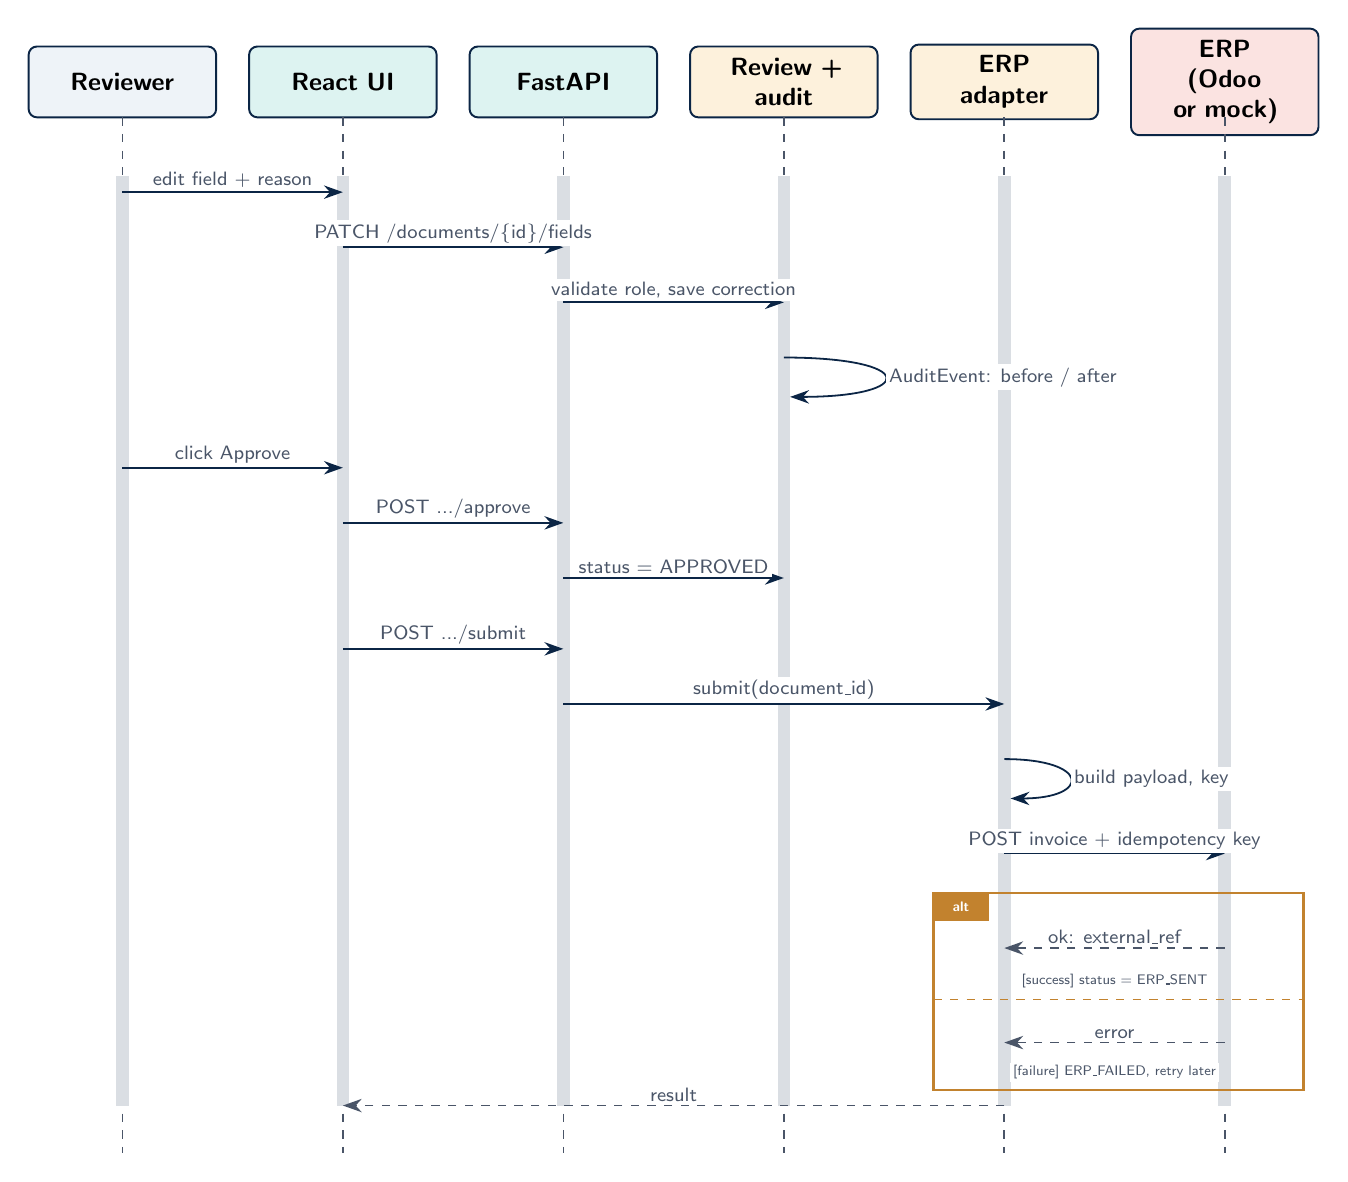
\begin{tikzpicture}[x=1cm,y=1cm]
\foreach \x/\n/\c in {0.9/Reviewer/mist, 3.7/React UI/mint, 6.5/FastAPI/mint, 9.3/Review +\\audit/sand, 12.1/ERP\\adapter/sand, 14.9/ERP\\(Odoo or mock)/blush}{
  \node[box,fill=\c,minimum width=2.3cm,text width=2.1cm,minimum height=0.9cm] at (\x,0) {\textbf{\n}};
  \draw[lifeline] (\x,-0.45) -- (\x,-13.6);
  \fill[navy!15] (\x-0.08,-1.2) rectangle (\x+0.08,-13.0);}
\draw[msg] (0.9,-1.4) -- node[lbl,above]{edit field + reason} (3.7,-1.4);
\draw[msg] (3.7,-2.1) -- node[lbl,above]{PATCH /documents/\{id\}/fields} (6.5,-2.1);
\draw[msg] (6.5,-2.8) -- node[lbl,above]{validate role, save correction} (9.3,-2.8);
\draw[msg] (9.3,-3.5) .. controls (11,-3.5) and (11,-4.0) .. node[lbl,right,pos=0.5]{AuditEvent: before / after} (9.38,-4.0);
\draw[msg] (0.9,-4.9) -- node[lbl,above]{click Approve} (3.7,-4.9);
\draw[msg] (3.7,-5.6) -- node[lbl,above]{POST .../approve} (6.5,-5.6);
\draw[msg] (6.5,-6.3) -- node[lbl,above]{status = APPROVED} (9.3,-6.3);
\draw[msg] (3.7,-7.2) -- node[lbl,above]{POST .../submit} (6.5,-7.2);
\draw[msg] (6.5,-7.9) -- node[lbl,above]{submit(document\_id)} (12.1,-7.9);
\draw[msg] (12.1,-8.6) .. controls (13.2,-8.6) and (13.2,-9.1) .. node[lbl,right,pos=0.5]{build payload, key} (12.18,-9.1);
\draw[msg] (12.1,-9.8) -- node[lbl,above]{POST invoice + idempotency key} (14.9,-9.8);
% alt frame
\draw[amber!80!black,line width=0.8pt] (11.2,-10.3) rectangle (15.9,-12.8);
\fill[amber!80!black] (11.2,-10.3) rectangle (11.9,-10.65);
\node[text=white,font=\sffamily\bfseries\tiny] at (11.55,-10.47) {alt};
\draw[ret] (14.9,-11.0) -- node[lbl,above]{ok: external\_ref} (12.1,-11.0);
\node[font=\sffamily\tiny,text=slate,fill=white,inner sep=1pt] at (13.5,-11.42) {[success] status = ERP\_SENT};
\draw[dashed,amber!80!black] (11.2,-11.65) -- (15.9,-11.65);
\draw[ret] (14.9,-12.2) -- node[lbl,above]{error} (12.1,-12.2);
\node[font=\sffamily\tiny,text=slate,fill=white,inner sep=1pt] at (13.5,-12.58) {[failure] ERP\_FAILED, retry later};
\draw[ret] (12.1,-13.0) -- node[lbl,above]{result} (3.7,-13.0);
\end{tikzpicture}
}
\caption{Review, approval and ERP submission.}\label{fig:p2seqreview}
\end{figure}
\begin{enumerate}
\item The service checks that the status is APPROVED or ERP\_FAILED and locks the document row.
\item It runs \texttt{check\_payload}. Any BLOCKING finding stops the submission before anything is sent and the status stays APPROVED.
\item It inserts an \texttt{erp\_attempts} row (PENDING) with the next attempt number and the key \texttt{idp-<document\_\allowbreak id>}, then commits.
\item It calls \texttt{submit}. On success the attempt becomes SENT with the ERP reference and the document becomes ERP\_SENT. On failure the attempt becomes FAILED with a category and the document becomes ERP\_FAILED.
\item To our knowledge Odoo has no built-in idempotency-key header. Before creating a bill on a retry, the Odoo adapter therefore searches for an existing bill with the same vendor reference and partner and, if found, returns it as success. This behaviour must be confirmed against the real ERP.
\end{enumerate}

\subsection{Errors and retries}
{\tblstart\small
\begin{longtable}{L{2.6cm}L{4.6cm}L{6.6cm}}
\hdrrow \hdr{Category} & \hdr{Example} & \hdr{Handling (values provisional)}\\ \endhead
AUTH & Wrong or expired ERP key. & No automatic retry; alert the administrator; document stays ERP\_FAILED.\\
VALIDATION & ERP refuses a value. & No automatic retry; reviewer corrects the data, then submits again.\\
TIMEOUT & No answer in time. & Retry up to three times with growing delay, same key; the pre-send search prevents a duplicate.\\
SERVER & ERP error 5xx. & Same as timeout.\\
DUPLICATE & A bill with this reference exists. & Treated as success and the existing reference is stored.\\
\hline
\end{longtable}}

\subsection{Mock ERP contract}
The mock accepts \texttt{POST /vendor-bills} with an \texttt{Idempotency-Key} header. A new key returns \texttt{201} and a reference. A repeated key returns \texttt{200} with the same reference and creates nothing. Switches in the request let tests force a timeout, a \texttt{401} and a validation error. The same test suite runs against the mock now and against Odoo when it is available.

% =====================================================================
\chapter{Traceability, Open Decisions and Next Steps}\label{ch:p2trace}
\section{Acceptance criteria of the six stories}
``Designed'' means the design is written in this document or in a companion file. ``Checked'' means a program verified part of it. It does not mean implemented.
{\tblstart\footnotesize
\begin{longtable}{L{1.1cm}L{5.0cm}L{2.0cm}L{5.7cm}}
\hdrrow \hdr{Story} & \hdr{Acceptance criterion} & \hdr{Where} & \hdr{State}\\ \endhead
US-06 & React + Vite as frontend. & Ch.~\ref{ch:p2arch} & Designed.\\
US-06 & FastAPI as backend API. & Ch.~\ref{ch:p2arch} & Designed; health endpoints exist and are tested.\\
US-06 & MySQL as relational database. & Ch.~\ref{ch:p2arch}, \ref{ch:p2db} & Designed; schema checked on MariaDB.\\
US-06 & OCR pipeline and ERP integration in a diagram. & Fig.~\ref{fig:p2arch}, \ref{fig:p2pipeline} & Designed.\\
US-07 & Required entities identified. & Ch.~\ref{ch:p2db} & Designed (\nTables{} tables).\\
US-07 & Tables for documents, extracted fields, review decisions. & Ch.~\ref{ch:p2db} & Designed and checked.\\
US-07 & Primary keys, foreign keys, relationships. & Fig.~\ref{fig:p2er} & Designed and checked (nine negative tests).\\
US-07 & Processing status and audit history. & Ch.~\ref{ch:p2db} & Designed and checked (status values, append-only trigger).\\
US-08 & Upload and file validation. & Sec.~\ref{sec:p2upload} & Designed.\\
US-08 & Preprocessing and OCR. & Stages 4--5 & Designed; not built.\\
US-08 & Extraction and confidence scoring. & Stages 6--7 & Designed; thresholds provisional.\\
US-08 & Human review of uncertain results. & Ch.~\ref{ch:p2flow} & Designed.\\
US-08 & Approved path to ERP. & Stage 10, Ch.~\ref{ch:p2sec} & Designed.\\
US-09 & Upload and retrieval endpoints. & Ch.~\ref{ch:p2api} & Designed and checked (contract validates).\\
US-09 & Endpoints for fields and review decisions. & Ch.~\ref{ch:p2api} & Designed and checked.\\
US-09 & Response formats and error handling. & Ch.~\ref{ch:p2api} & Designed.\\
US-09 & Authentication and authorisation. & Ch.~\ref{ch:p2api} & Designed; token lifetime open.\\
US-10 & Dashboard sketch. & Fig.~\ref{fig:p2dash} & Designed.\\
US-10 & Upload page. & Fig.~\ref{fig:p2upload} & Designed.\\
US-10 & Extraction results and review screens. & Fig.~\ref{fig:p2review} & Designed.\\
US-10 & Loading, success and error states. & Ch.~\ref{ch:p2ui} & Designed.\\
US-11 & Access permissions and credential management. & Ch.~\ref{ch:p2api}, \ref{ch:p2sec} & Designed.\\
US-11 & File validation and data protection. & Sec.~\ref{sec:p2upload}, Ch.~\ref{ch:p2sec} & Designed.\\
US-11 & \textbf{Target Odoo version and available API.} & Ch.~\ref{ch:p2sec} & \textbf{Not closed.} Options documented; needs the real version (P2-D1).\\
US-11 & Validation and error handling before ERP submission. & Ch.~\ref{ch:p2sec} & Designed.\\
\hline
\end{longtable}}

\section{Open decisions}\label{sec:p2open}
{\tblstart\small
\begin{longtable}{L{1.4cm}L{6.4cm}L{6.0cm}}
\hdrrow \hdr{ID} & \hdr{Decision needed} & \hdr{Effect}\\ \endhead
P2-D1 & Which Odoo version and access (cloud, on-premise, test instance)? & Chooses JSON-2 or XML-RPC adapter; closes US-11.\\
P2-D2 & Token lifetime, and whether to add refresh tokens. & Changes the login endpoint and the frontend client.\\
P2-D3 & May a reviewer approve a document they uploaded themselves? & Adds a separation-of-duties check to approval.\\
P2-D4 & Retention period and deletion procedure for documents. & Defines use of \texttt{deleted\_at} and a clean-up job.\\
P2-D5 & Post vendor bills in the ERP, or leave them in draft? & Changes the final ERP call.\\
P2-D6 & Final thresholds and tolerances. & Set only after the OCR baseline exists.\\
\hline
\end{longtable}}
The open decisions D1 to D9 of the Phase 1 document still apply; in particular the document type scope (D3), the dataset (D6) and the training hardware (D7).

\section{Risks specific to this phase}
{\tblstart\small
\begin{longtable}{L{4.4cm}L{4.4cm}L{5.0cm}}
\hdrrow \hdr{Risk} & \hdr{Effect} & \hdr{Mitigation}\\ \endhead
Odoo version differs from the assumption & ERP adapter must be rewritten. & Adapter interface; mock first; decide P2-D1 early.\\
Models, migrations and \texttt{schema.sql} drift apart & Wrong schema in some environments. & Compare the migrated database with \texttt{schema.sql} in a test.\\
API code drifts from the contract & React and backend disagree. & Compare the generated schema with \texttt{openapi.yaml}; contract tests.\\
Schema tested only on MariaDB & A MySQL 8.0 difference appears late. & Run the file on MySQL 8.0 as the first Phase 3 task.\\
Design too large for the time available & Late features missing. & Build in the order of Chapter~\ref{ch:p2trace}; line items and the admin screens can be reduced.\\
\hline
\end{longtable}}

\section{Next steps}
The next phase is the development environment and the working foundation (stories US-12 to US-16). The design above gives it this order of work.
\begin{enumerate}
\item Confirm that the Phase 1 backend runs on the developer's PC (health and database checks).
\item Run \texttt{schema.sql} on MySQL 8.0 and fix any difference.
\item Write the SQLAlchemy models and the first Alembic revision, including the checks and triggers; compare the migrated schema with \texttt{schema.sql}.
\item Install and verify OpenCV and PyTorch, and set up the React and Vite application.
\item Implement sign-in with roles, then upload with file validation, then the status endpoints, each with tests, keeping \texttt{openapi.yaml} in step.
\end{enumerate}

\appendix
\chapter{Database Schema Listing}
The complete file \texttt{schema.sql}, as it was loaded and tested.
{\lstset{basicstyle=\ttfamily\tiny,language=SQL}
\lstinputlisting{/home/claude/phase2/schema.sql}}


\end{document}
